\chapter{Evolutionary Patterns of Group B Sox Binding in \emph{Drosophila}}

\hrulefill

\section{Overview and motivation}

While many aspects of Dichaete and SoxN function can be understood by examining the DamID datasets that I generated in each species independently, a comparative approach that looks at binding through the lens of natural selection has the potential to reveal a more nuanced view. The turnover of transcription factor binding sites between species is a well-documented phenomenon in both flies and vertebrates, although, most likely due to the compact genome and large effective population sizes, a greater percentage of binding sites are generally conserved between different species of \emph{Drosophila} than between mammals at a similar evolutionary distance \citep{bradley_binding_2010,he_high_2011,odom_tissue-specific_2007,schmidt_five-vertebrate_2010,stefflova_cooperativity_2013,villar_evolution_2014}. This is a useful feature, as it facilitates the identification of binding sites that have potentially been subject to selective pressure. In theory, binding events that are more functionally important will be subject to greater constraint under purifying selection and will therefore tend to be conserved between species. However, not all non-conserved sites are non-functional; the evolution of new binding sites can be driven by positive selection either to compensate for the loss of a site elsewhere or in connection with a new function \citep{arnoult_emergence_2013,frankel_conserved_2012,he_does_2011,kalay_nomadic_2010}. For Dichaete and SoxN, a number of different questions can be asked using comparative binding data, including whether certain genomic features or functional categories of genes are associated with conserved binding events for each TF, what is the relationship is between Dichaete and SoxN binding overlap and conservation of binding between species, and how changes in the sequence or number of Sox motifs within intervals are associated with binding conservation or divergence. I used comparisons between the binding patterns of the two TFs as well as the binding patterns of each TF between multiple species to try to answer these questions.\\

The evolutionary conservation of transcription factor binding sites can be studied on several levels: the qualitative presence or absence of a binding interval, quantitative measures of binding affinity, or the underlying DNA sequence and motifs. I have attempted to address all of these levels of conservation to build a detailed picture of the evolutionary dynamics of Dichaete and SoxN binding in \emph{Drosophila}. In this chapter, I start by performing quantitative pairwise comparisons of Dichaete and SoxN binding patterns between \emph{D. melanogaster} and each of the other species for which I have data. This provides a more detailed view of the similarities and differences between binding datasets than a simple intersection of binding intervals. I also perform a three-way quantitative comparison of Dichaete-Dam binding in \emph{D. melanogaster, D. simulans} and \emph{D. yakuba}. In order to address the relationship between Dichaete and SoxN binding, I use both qualitative and quantitative measures to examine whether there is any difference in conservation rates between intervals that are bound uniquely by Dichaete-Dam or SoxN-Dam in different species and those that are bound commonly by both TFs. Zooming out to the gene level, I examine possible instances of binding site turnover and compensatory evolution within gene loci. If Dichaete and SoxN binding at known enhancers and core intervals is truly functional, one would expect it to show increased levels of conservation; I also examine this hypothesis using qualitative measures of binding conservation.\\

Finally, I search for Sox motifs located within intervals and examine the relationship between motif number and quality and binding conservation. This analysis focuses primarily on the Dichaete-Dam binding intervals, as there is a Dichaete-Dam dataset available in all four species studied. Although the number of fully conserved binding intervals is small compared to the total number of binding intervals identified, in part due to the smaller number of intervals identified in \emph{D. pseudoobscura}, the functional analyses performed in the previous chapter indicate that these are high-confidence binding intervals enriched for high-quality Sox motifs, and are thus useful for drawing conclusions about the effect of motif presence and quality on TF binding. In addition to searching for Sox motifs in conserved and non-conserved binding intervals, I also perform multiple alignments of binding intervals to examine positional and nucleotide-level motif conservation in the context of both qualitative and quantitative changes in binding. Details of the computational methods used to perform evolutionary analyses can be found in Chapter 2.

\section{Pairwise comparison of binding between \emph{D. melanogaster} and non-model species}

Finding the overlap between binding intervals gives a rough estimate of the conservation of binding events between species; however, this does not take into account the strength of binding within intervals. It is also likely to be overly conservative due to the fact that the variance differs between the different sets of replicates, resulting in different effective thresholds for detection of enriched binding at a given p-value. In order to get a more nuanced view of conserved and differential binding between \emph{D. melanogaster} and each other species, I used DiffBind to perform a comparative analysis, using the translated reads and peaks called from translated reads for all non-\emph{melanogaster} species \citep{ross-innes_differential_2012-1}.

\subsection{Quantitative comparison of binding between \emph{D. melanogaster} and \emph{D. simulans}}

Using DiffBind to cluster both the Dichaete-Dam and SoxN-Dam binding interval datasets for \emph{D. melanogaster} and \emph{D. simulans}, one can observe that, in general, the SoxN-Dam replicates from both species cluster together and the Dichaete-Dam replicates from both species cluster together (Figure 5.1). Replicate 1 of SoxN-Dam in \emph{D. melanogaster} is an exception to this pattern, as it clusters more closely to replicate 1 of Dichaete-Dam in \emph{D. melanogaster}; this may be due to an effect of the sequencing platform, since these two replicates were sequenced on a MiSeq while all of the others were sequenced on a HiSeq. In general, the binding profiles for Dichaete-Dam and SoxN-Dam in \emph{D. melanogaster} appear more similar than the binding profiles for Dichaete-Dam and SoxN-Dam in \emph{D. simulans}.\\

\begin{figure}
\centering
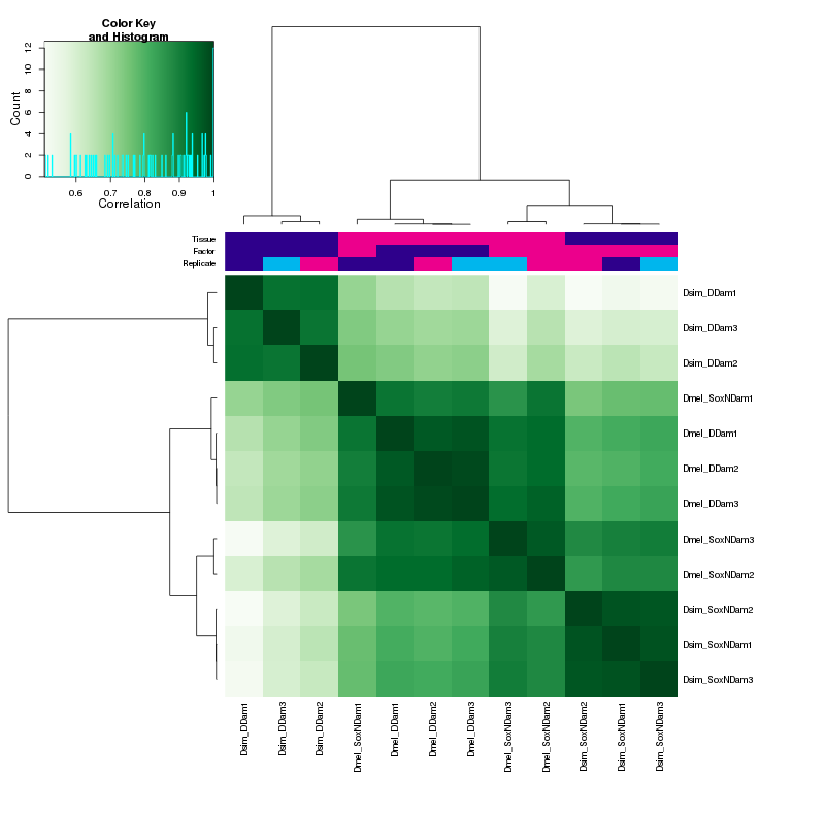
\includegraphics{fig5-1}
\caption{Clustering of \emph{D. melanogaster} and \emph{D. simulan}s Dichaete-Dam and SoxN-Dam samples by binding affinity scores in all bound intervals. Both the Dichaete-Dam replicates  from both species and the SoxN-Dam replicates from both species tend to cluster together, with the exception of \emph{D. melanogaster} SoxN-Dam replicate 1. The color key and histogram shows the distribution of correlation coefficients for affinity scores in each pair of samples. Darker green corresponds to a higher correlation between samples, while lighter green corresponds to a lower correlation.}
\label{Figure 5.1}
\end{figure}

Examining the data for one transcription factor at a time highlights the differences between species (Figure 5.2). For Dichaete-Dam, a total of 23985 binding intervals were considered in both species. There is a clear division between the two species. The three \emph{D. melanogaster} replicates are highly similar, while in \emph{D. simulans}, replicate 3 is a slight outlier. Comparing each \emph{D. melanogaster} replicate with each \emph{D. simulans} replicate, the correlations of binding profiles at all bound peaks between the two species range from 0.62 - 0.72, while the correlations of replicates within a single species range from 0.92 - 0.93 for \emph{D. simulans} and from 0.97 - 0.99 for \emph{D. melanogaster}. 11596 binding intervals were identified as differentially enriched between the two species at FDR10 using DESeq2 normalization. For further analysis, I decided to use a stringent set of binding intervals that were called as differentially bound between \emph{D. melanogaster} and \emph{D. simulans} at FDR1. This set contains 7246 binding intervals, representing 45.0\% of all \emph{D. simulans} bound intervals and 34.8\% of all \emph{D. melanogaster} bound intervals (Figure 5.3).\\

Of these, 4039 are preferentially bound in \emph{D. simulans} and 3207 are preferentially bound in \emph{D. melanogaster}. Clustering the differentially bound intervals by affinity scores reveals two large blocks of intervals that are highly bound in only either \emph{D. melanogaster} or \emph{D. simulans} (Figure 5.4); these could be considered as gains or losses of binding events in each lineage. In addition, there are smaller clusters of intervals that have high affinity scores in both species, but are more highly bound in one than the other. These intervals represent binding events present in both species whose strength has changed quantitatively during evolution. All of the intervals called as preferentially bound in \emph{D. simulans} were also identified as bound by \emph{D. simulans} in the single-species DESeq2 analysis. Of these intervals, 1885 were also called as binding intervals at FDR5 in \emph{D. melanogaster} in the single-species analysis, while 2154 were not. All but three of the intervals called as preferentially bound in \emph{D. melanogaster} were called as binding intervals in the single-species analysis; this slight discrepancy results from normalizing the reads from both species together before performing the differential analysis. 1026 of these were also called as binding intervals at FDR5 in \emph{D. simulans} in the single-species analysis, while 2178 were not.\\

\begin{figure}
\centering
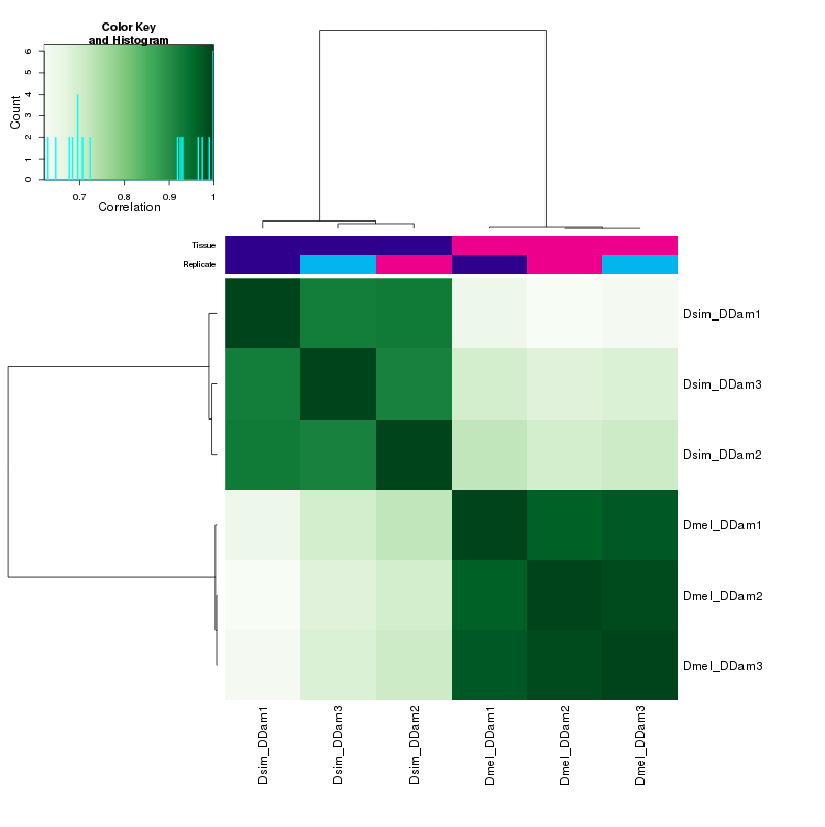
\includegraphics{fig5-2}[H]
\caption{Clustering of \emph{D. melanogaster} and \emph{D. simulans} Dichaete-Dam samples by binding affinity scores in all bound intervals. Biological replicates from each species cluster strongly together. The color key and histogram shows the distribution of correlation coefficients for affinity scores in each pair of samples. Darker green corresponds to a higher correlation between samples, while lighter green corresponds to a lower correlation.}
\label{Figure 5.2}
\end{figure}

\begin{figure}
\centering
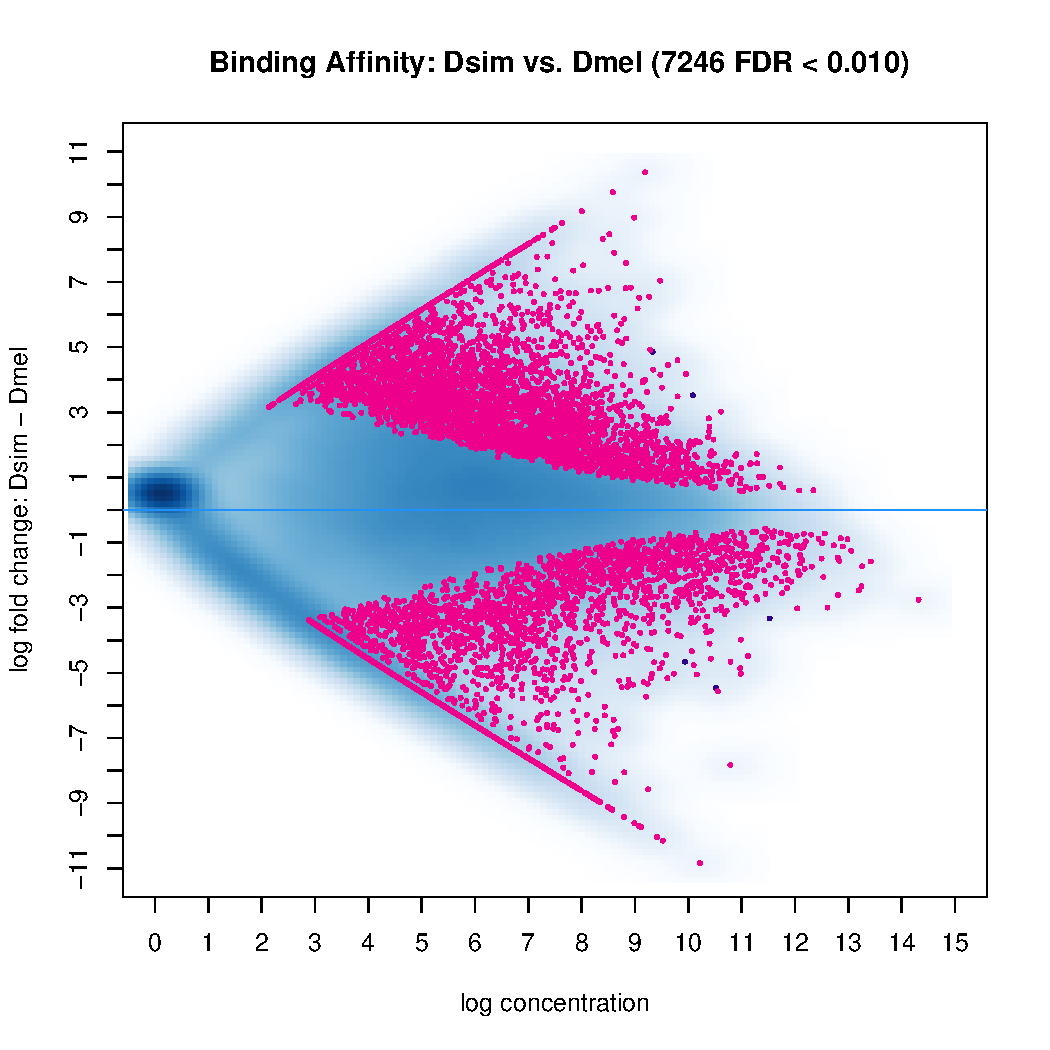
\includegraphics[width=13.97cm]{fig5-3}
\caption{MA plot showing differentially bound intervals with FDR \textless 0.01 between \emph{D. melanogaster} Dichaete-Dam and \emph{D. simulans} Dichaete-Dam. Intervals that are bound more strongly in \emph{D. simulans} have a positive log fold change, while intervals that are bound more strongly in \emph{D. melanogaster} have a negative log fold change. All intervals are plotted; differentially bound intervals are highlighted in pink.}
\label{Figure 5.3}
\end{figure}

\begin{figure}
\centering
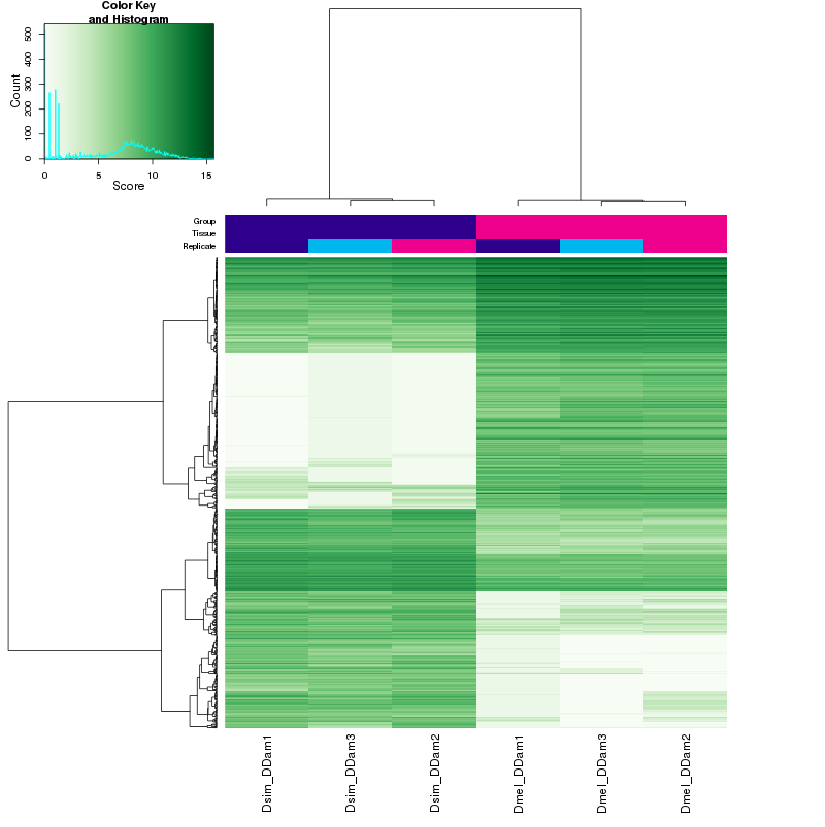
\includegraphics{fig5-4}
\caption{Clustering of \emph{D. simulans} and \emph{D. melanogaster} Dichaete-Dam differentially bound intervals by binding affinity scores. Roughly similar numbers of intervals are preferentially bound in each species. The color key and histogram shows the distribution of binding affinity scores (log of normalized read counts), in all bound intervals in each sample. Darker green corresponds to higher affinity scores or stronger binding, while lighter green corresponds to lower affinity scores or weaker binding.}
\label{Figure 5.4}
\end{figure}

For SoxN-Dam, a total of 24794 binding intervals were considered in both species. As with Dichaete-Dam, the replicates from each species cluster closely together. In this case, the three \emph{D. simulans} replicates are the most similar, while the biggest outlier is replicate 1 for \emph{D. melanogaster} (Figure 5.5). The correlations between binding profiles between \emph{D. melanogaster} and \emph{D. simulans} range from 0.75 - 0.90, while the correlations for replicates within a species range from 0.97 - 0.98 for \emph{D. simulans} and from 0.87 - 0.97 for \emph{D. melanogaster}. Using DESeq2 normalization, DiffBind identifies 9278 differentially bound intervals between the two species at FDR10. A high-confidence set of differentially bound intervals identified at FDR1 contains 4923 binding intervals (Figure 5.6), representing 32.5\% of all \emph{D. simulans} bound intervals and 21.4\% of all \emph{D. melanogaster} bound intervals. Of these, 2412 are preferentially bound in \emph{D. simulans}, while 2511 are differentially bound in \emph{D. melanogaster}. Clustering the differentially bound intervals by affinity score reveals that, as with Dichaete, the largest groups of intervals are highly bound only in either \emph{D. melanogaster} or \emph{D. simulans}; smaller blocks of intervals are bound in both species but more highly in one than in the other (Figure 5.7). Of the 2412 intervals that are preferentially bound in \emph{D. simulans}, 2407 were called as binding intervals at FDR5 in the single-species analysis. 1101 of these were also called as bound at FDR5 in \emph{D. melanogaster}, while 1306 were not. In this case, all 2511 intervals that are preferentially bound in \emph{D. melanogaster} were called as binding intervals in the single-species analysis. Only 363 of these were also called as bound at FDR5 in \emph{D. simulans}, while 2148 were not.

\begin{figure}
\centering
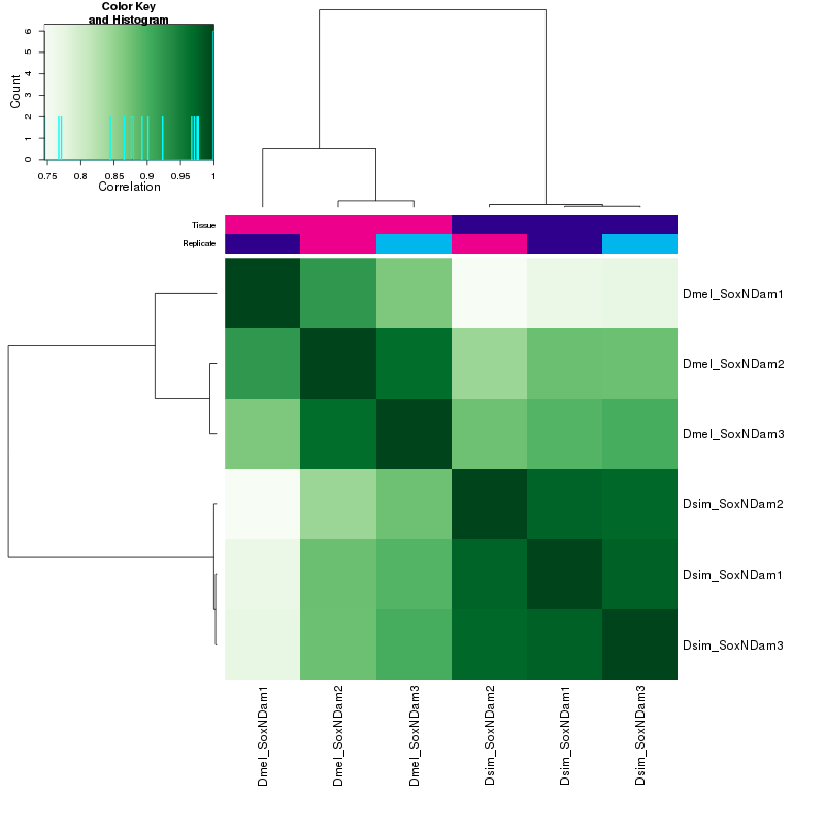
\includegraphics{fig5-5}
\caption{Clustering of \emph{D. melanogaster} and \emph{D. simulans} SoxN-Dam samples by binding affinity score in all bound intervals. Biological replicates from each species cluster together, although the \emph{D. simulans} replicates show stronger correlations than the \emph{D. melanogaster} replicates. The biggest outlier is \emph{D. melanogaster} replicate 1. The color key and histogram shows the distribution of correlation coefficients for affinity scores in each pair of samples. Darker green corresponds to a higher correlation between samples, while lighter green corresponds to a lower correlation.}
\label{Figure 5.5}
\end{figure}

\begin{figure}
\centering
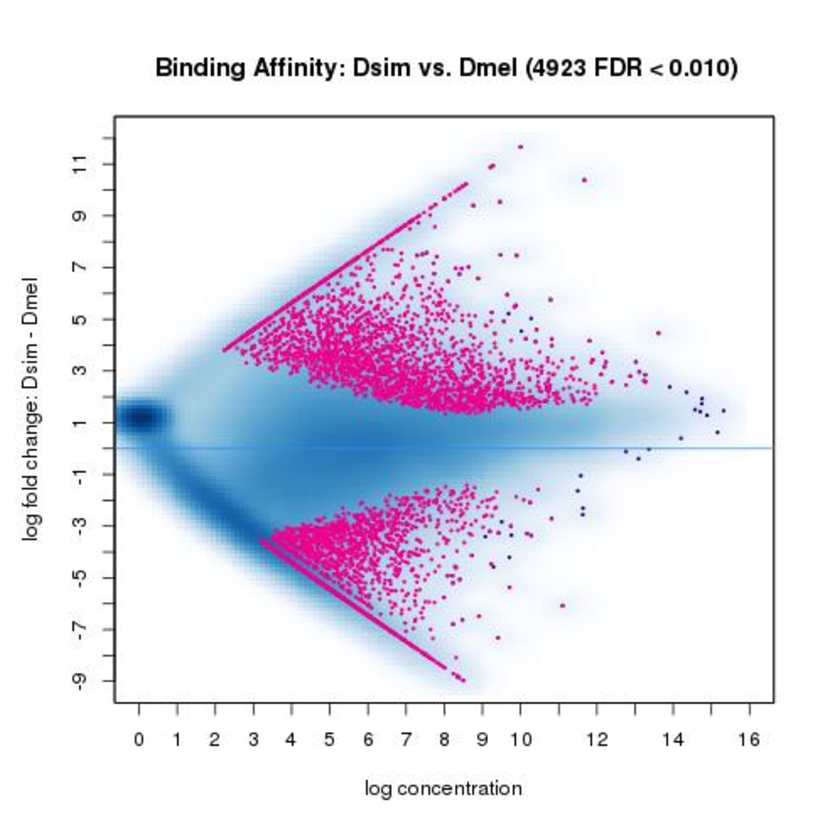
\includegraphics{fig5-6}
\caption{MA plot showing differentially bound intervals with FDR \textless 0.01 between \emph{D. simulans} SoxN-Dam and \emph{D. melanogaster} SoxN-Dam. Intervals that are bound more strongly in \emph{D. simulans} have a positive log fold change, while intervals that are bound more strongly in \emph{D. melanogaster} have a negative log fold change. All intervals are plotted; differentially bound intervals are highlighted in pink.}
\label{Figure 5.6}
\end{figure}

\begin{figure}
\centering
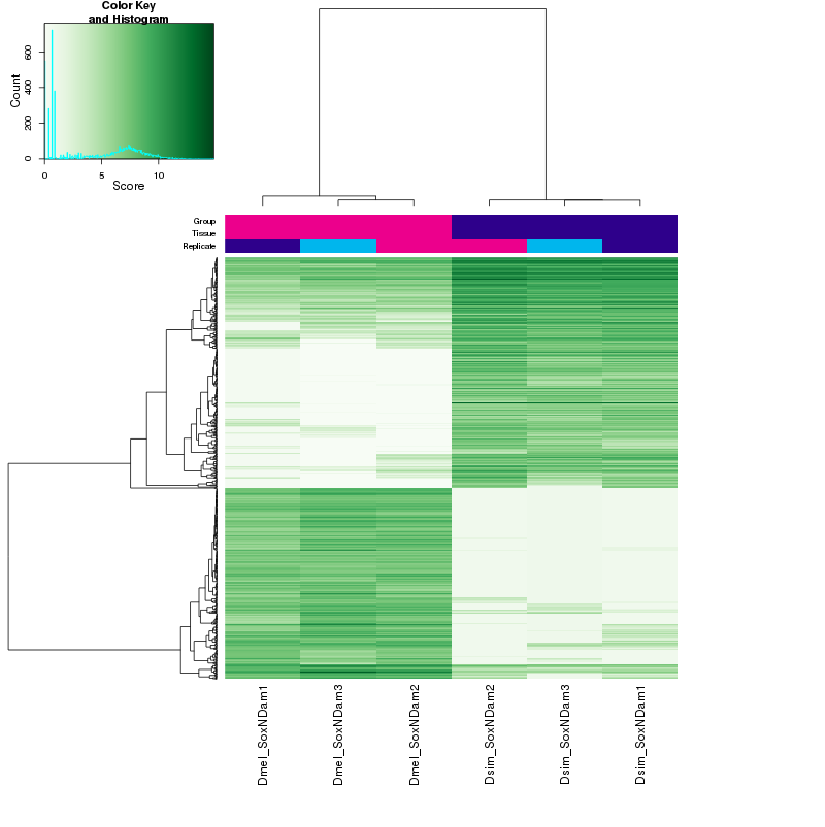
\includegraphics{fig5-7}
\caption{Clustering of \emph{D. melanogaster} and \emph{D. simulans} SoxN-Dam differentially bound intervals by binding affinity scores. Roughly similar numbers of intervals are preferentially bound in each species. The color key and histogram shows the distribution of binding affinity scores (log of normalized read counts), in all bound intervals in each sample. Darker green corresponds to higher affinity scores or stronger binding, while lighter green corresponds to lower affinity scores or weaker binding.}
\label{Figure 5.7}
\end{figure}

\subsection{Quantitative comparison of Dichaete binding between \emph{D. melanogaster} and \emph{D. yakuba}}
A total of 25072 unique binding intervals were considered by DiffBind in the comparison between Dichaete-Dam binding in \emph{D. melanogaster} and \emph{D. yakuba}. As with the Dichate-Dam data in \emph{D. simulans}, there is a clear division between the binding intervals in \emph{D. yakuba} and those in \emph{D. melanogaster}, with the replicates from each species clustering closely together (Figure 5.8). The correlation coefficients between replicates from different species range from 0.68 - 0.70, while the correlation coefficients between replicates from the same species range from 0.96 - 0.99, showing a very high degree of reproducibility. 13620 binding intervals were identified as differentially bound between the two species using DESeq2 normalization at FDR10. A more stringent, high-confidence set of differentially bound intervals at FDR1 contains 9205 binding intervals (Figure 5.9), representing 43.9\% of all \emph{D. yakuba} bound intervals and 44.2\% of all \emph{D. melanogaster} bound intervals. Of these, 4383 are preferentially bound in \emph{D. yakuba} and 4822 are preferentially bound in \emph{D. melanogaster}. Clustering the differentially bound intervals by affinity score reveals that, of those intervals preferentially bound in \emph{D. yakuba}, the majority are also bound at a lower level in \emph{D. melanogaster}, while a smaller number are unique to \emph{D. yakuba} (Figure 5.10). Conversely, of those intervals preferentially bound in \emph{D. melanogaster}, the majority are unique to that species, while a smaller number are also bound by \emph{D. yakuba} at a lower level. Of the Dichaete-Dam intervals preferentially bound in \emph{D. yakuba}, all but 2 were called as bound intervals at FDR5 in the single-species DESeq2 analysis. 2301 of these were also called as bound at FDR5 by \emph{D. melanogaster}, while 2080 were not. Of the 4822 intervals preferentially bound in \emph{D. melanogaster}, 4783 were called as bound intervals at FDR5 in the single-species analysis. 2193 of these were also called as bound at FDR5 in \emph{D. yakuba}, while 2590 were unique to \emph{D. melanogaster}.

\begin{figure}
\centering
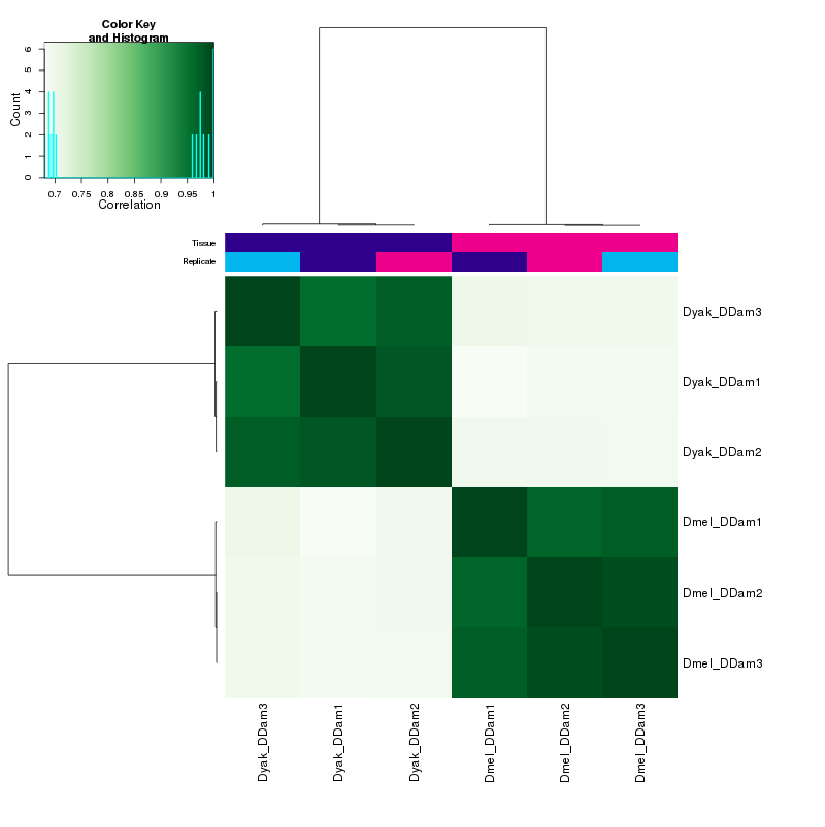
\includegraphics{fig5-8}
\caption{Clustering of \emph{D. melanogaster} and \emph{D. yakuba} Dichaete-Dam samples by binding affinity scores in all bound intervals. Biological replicates from each species cluster strongly together. The color key and histogram shows the distribution of correlation coefficients for affinity scores in each pair of samples. Darker green corresponds to a higher correlation between samples, while lighter green corresponds to a lower correlation.}
\label{Figure 5.8}
\end{figure}

\begin{figure}
\centering
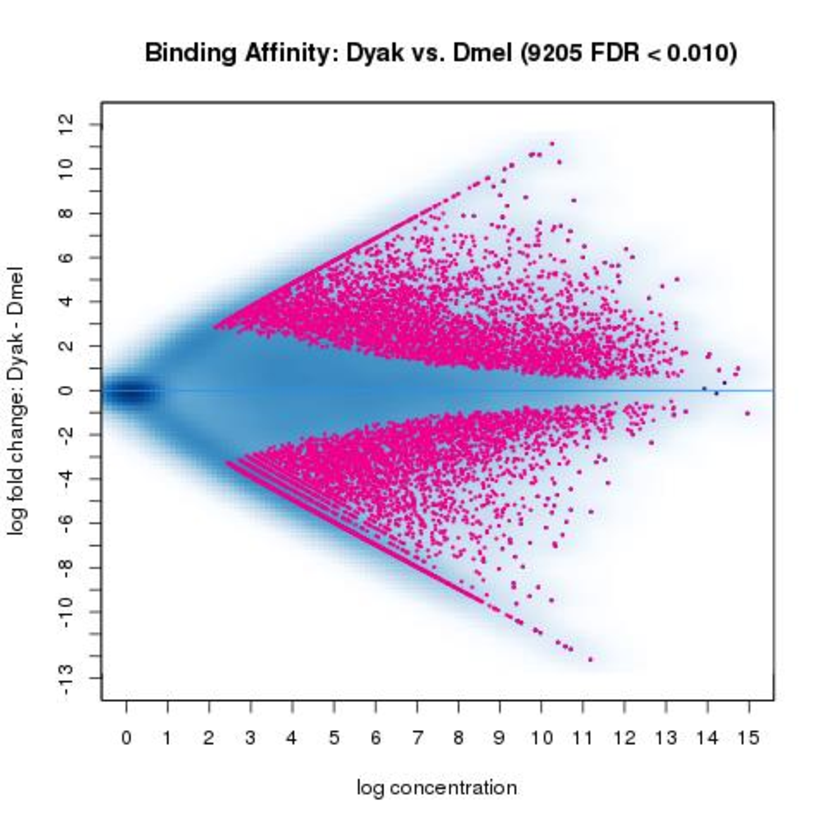
\includegraphics{fig5-9}
\caption{MA plot showing differentially bound intervals with FDR \textless 0.01 between \emph{D. melanogaster} Dichaete-Dam and \emph{D. yakuba} Dichaete-Dam. Intervals that are bound more strongly in \emph{D. yakuba} have a positive log fold change, while intervals that are bound more strongly in \emph{D. melanogaster} have a negative log fold change. All intervals are plotted; differentially bound intervals are highlighted in pink.}
\label{Figure 5.9}
\end{figure}

\begin{figure}
\centering
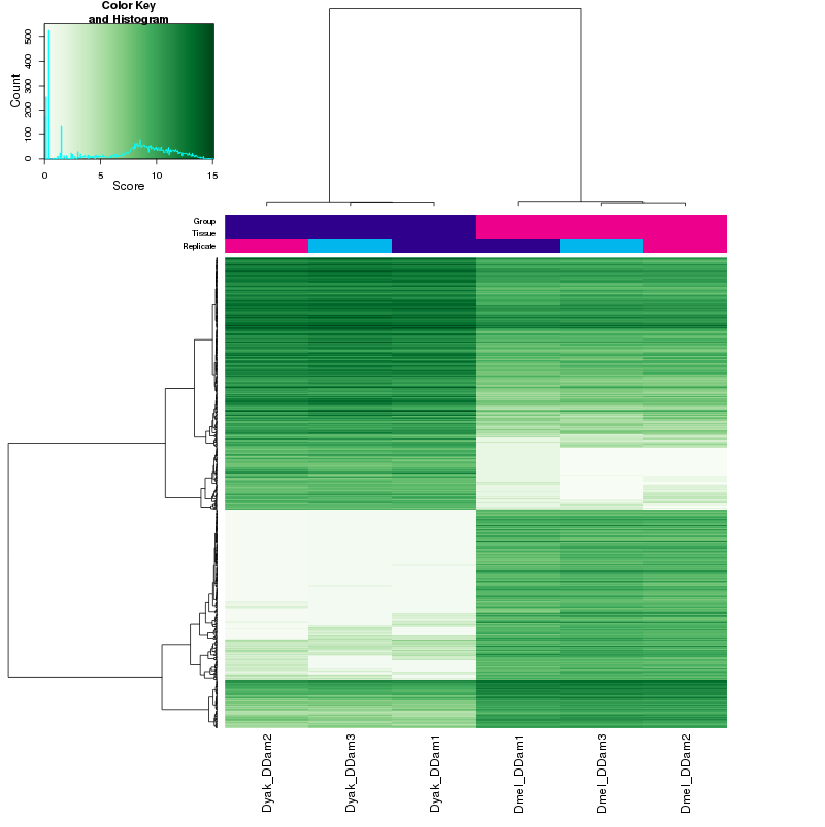
\includegraphics{fig5-10}
\caption{Clustering of \emph{D. yakuba} and \emph{D. melanogaster} Dichaete-Dam differentially bound intervals by binding affinity scores. Roughly similar numbers of intervals are preferentially bound in each species; however, the majority of intervals that are preferentially bound by \emph{D. melanogaster} are not bound in \emph{D. yakuba} (bottom half), while the majority of intervals that are preferentially bound in \emph{D. yakuba} are also bound in \emph{D. melanogaster} (top half). The color key and histogram shows the distribution of binding affinity scores (log of normalized read counts), in all bound intervals in each sample. Darker green corresponds to higher affinity scores or stronger binding, while lighter green corresponds to lower affinity scores or weaker binding.}
\label{Figure 5.10}
\end{figure}

\subsection{Quantitative comparison of Dichaete binding between \emph{D. melanogaster} and \emph{D. pseudoobscura}}
A total of 21294 unique binding intervals were considered by DiffBind in the comparison between Dichaete-Dam binding in \emph{D. pseudoobscura} and \emph{D. melanogaster}. The three replicates from each species cluster together; however, as expected given the noise present in the \emph{D. pseudoobscura} data, the correlations between \emph{D. pseudoobscura} replicates are much lower than those between \emph{D. melanogaster} replicates (Figure 5.11). The biggest outlier is clearly replicate 1 from \emph{D. pseudoobscura}. The correlation coefficients between replicates from \emph{D. pseudoobscura} range from 0.46 - 0.79, while the correlation coefficients between replicates from \emph{D. melanogaster} range from 0.96 - 0.99. The correlation coefficients between replicates from different species range from 0.46 - 0.72.\\

\begin{figure}
\centering
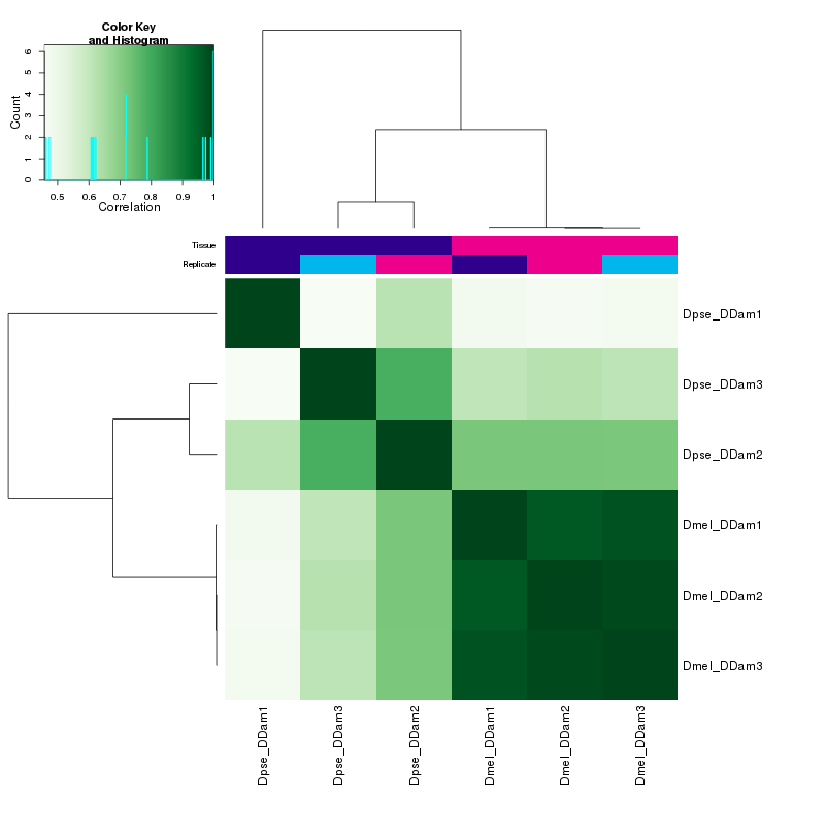
\includegraphics{fig5-11}
\caption{Clustering of \emph{D. melanogaster} and \emph{D. pseudoobscura} Dichaete-Dam samples by binding affinity scores in all bound intervals. Biological replicates from each species cluster  together, although the \emph{D. melanogaster} replicates are much more highly correlated than the \emph{D. pseudoobscura} replicates. The strongest outlier is \emph{D. pseudoobscura} replicate 1. The color key and histogram shows the distribution of correlation coefficients for affinity scores in each pair of samples. Darker green corresponds to a higher correlation between samples, while lighter green corresponds to a lower correlation.}
\label{Figure 5.11}
\end{figure}

This comparison presents a challenge for analysis, as, unlike the other pairwise comparisons between species, the two datasets are not of similar quality and do not contain similar numbers of binding intervals. In the previous DiffBind analyses using DESeq2, the sample affinity scores were normalized using only the reads present within binding intervals, as it could be assumed that the similar numbers of intervals present in the different samples reflected biological reality, and that most of the reads outside of those intervals represented background noise. However, that assumption was not valid in the case of the \emph{D. pseudoobscura} data. Since there are many less binding intervals in the \emph{D. pseudoobscura} dataset, normalizing by the number of reads within binding intervals would artificially inflate the affinity scores within those intervals relative to the ones present in the \emph{D. melanogaster} dataset. Accordingly, the sample affinity scores were normalized using the total library sizes of each sample. This may result in an underestimation of the number of significant preferentially enriched binding intervals in \emph{D. pseudoobscura}; however, it is the more conservative approach, and, as such, those intervals that are identified can be interpreted with high confidence.\\

\begin{figure}
\centering
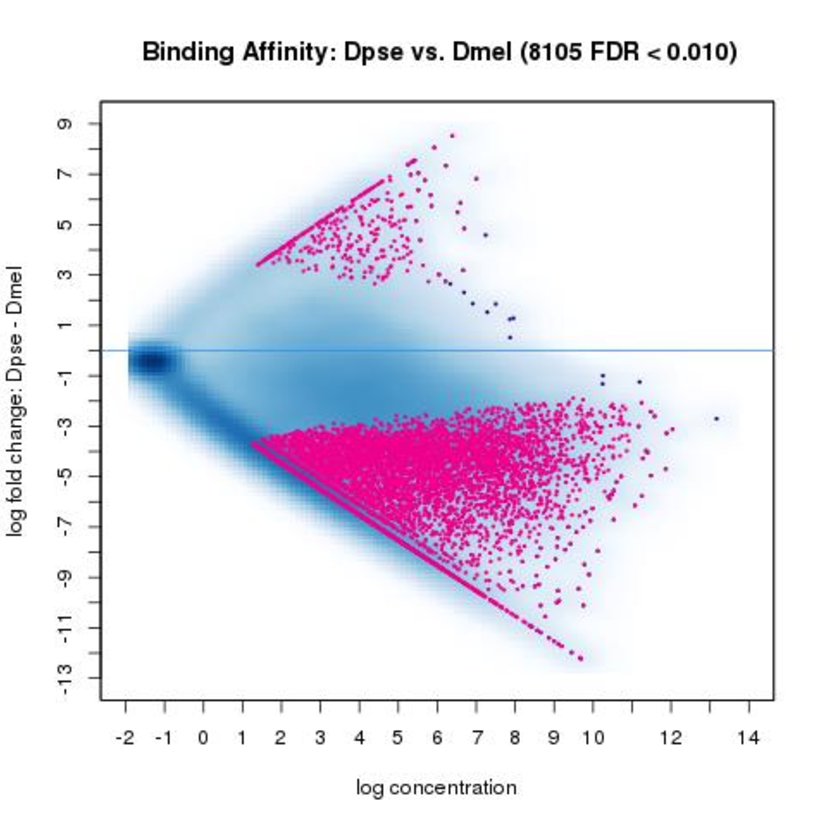
\includegraphics{fig5-12}
\caption{MA plot showing differentially bound intervals with FDR \textless 0.01 between \emph{D. melanogaster} Dichaete-Dam and \emph{D. pseudoobscura} Dichaete-Dam. Intervals that are bound more strongly in \emph{D. pseudoobscura} have a positive log fold change, while intervals that are bound more strongly in \emph{D. melanogaster} have a negative log fold change. All intervals are plotted; differentially bound intervals are highlighted in pink.}
\label{Figure 5.12}
\end{figure}

Using this method, 12227 binding intervals were identified as differentially bound between the two species at FDR10, and 8105 high-confidence intervals were identified at FDR1 (Figure 5.12). Of the FDR1 intervals, only 321 were preferentially bound in \emph{D. pseudoobscura}, while 7784 were preferentially bound in \emph{D. melanogaster}. Of the intervals preferentially bound in \emph{D. pseudoobscura}, 261 were called as binding intervals at FDR5 in the single-species DESeq2 analysis. 30 of these were also called as binding intervals at FDR5 in \emph{D. melanogaster}, while 231 were unique to \emph{D. pseudoobscura}. All of the intervals identified as preferentially bound in \emph{D. melanogaster} were called as binding intervals in the single-species DESeq2 analysis. Of these, 338 were also called as binding intervals at FDR5 in \emph{D. pseudoobscura}, while 7446 were unique to \emph{D. melanogaster}. Almost all of the intervals that are preferentially bound in one species are not bound in the other, which can be seen when all of the differentially bound intervals are clustered by affinity score (Figure 5.13). This is in contrast to the pairwise comparisons for Dichaete-Dam in the other two species, where a sizeable proportion of differentially bound intervals in one species are also bound in the other species, albeit at a lower level.

\begin{figure}
\centering
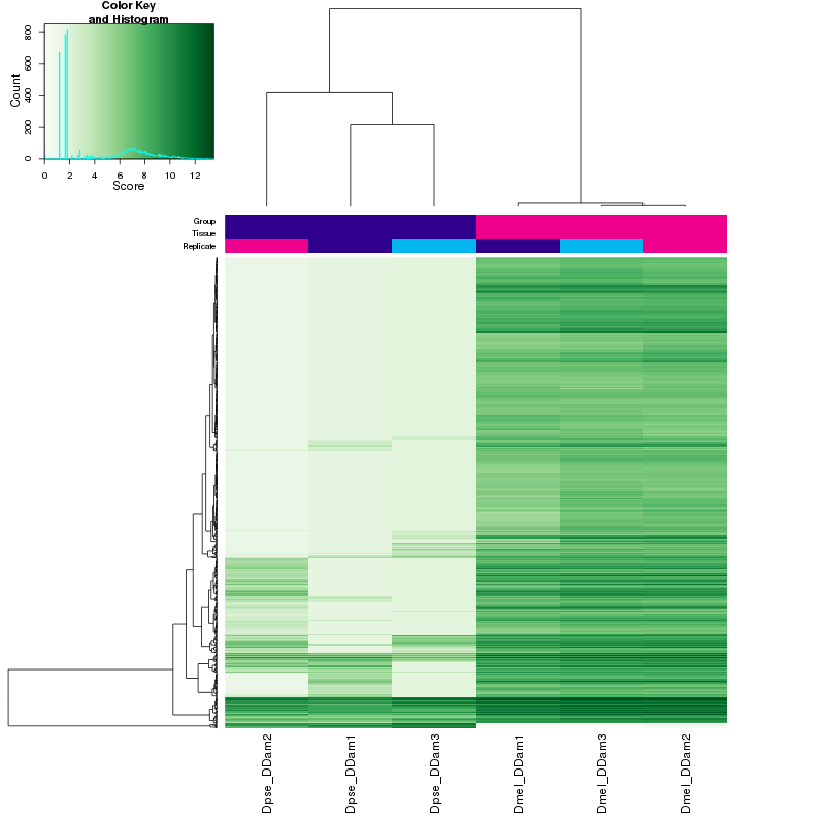
\includegraphics{fig5-13}
\caption{Clustering of \emph{D. pseudoobscura} and \emph{D. melanogaster} Dichaete-Dam differentially bound intervals by binding affinity scores. Many more intervals are preferentially bound in \emph{D. melanogaster} (right side) than in \emph{D. pseudoobscura} (left side) due to the higher noise and smaller number of intervals identified in \emph{D. pseudoobscura}. The color key and histogram shows the distribution of binding affinity scores (log of normalized read counts), in all bound intervals in each sample. Darker green corresponds to higher affinity scores or stronger binding, while lighter green corresponds to lower affinity scores or weaker binding}
\label{Figure 5.13}
\end{figure}

\subsection{Summary of pairwise binding divergence}
The numbers of Dichaete-Dam binding intervals called as differentially enriched between \emph{D. melanogaster} and each other species increase with phylogenetic distance from \emph{D. simulans} to \emph{D. yakuba}. Although less differential intervals are identified at FDR1 between \emph{D. melanogaster} and \emph{D. pseudoobscura} than between \emph{D. melanogaster} and \emph{D. yakuba}, the percentage of intervals that are unique to \emph{D. melanogaster} in comparison to \emph{D. pseudoobscura} is greater, and the number of intervals that are unique to \emph{D. pseudoobscura} are likely underestimated due to the normalization method employed. The total numbers of intervals identified as differentially bound in each comparison are summarized in Table 5.1. Interestingly, the proportions of binding intervals that are qualitatively absent in non-melanogaster species versus intervals that are present but have a quantitative change in binding strength vary between different species as well as between Dichaete and SoxN. For Dichaete-Dam, roughly equal percentages of the total binding intervals called in \emph{D. melanogaster} (20848) are qualitatively absent and present but quantitatively changed, either increasing or decreasing in binding strength, in \emph{D. simulans} (10.4\% and 10.6\%, respectively). However, while a similar proportion are qualitatively absent in \emph{D. yakuba} (12.4\%), roughly double the percentage of intervals are present but have quantitative changes in binding affinity (21.6\%). The proportion of \emph{D. melanogaster} intervals that are qualitatively absent in \emph{D. pseudoobscura}, 35.7\%, is likely exaggerated by the lower quality of the \emph{D. pseudoobscura} data; however, it is interesting that a much lower percentage of \emph{D. melanogaster} intervals are present but show quantitative changes in \emph{D. pseudoobscura} (1.8\%). It should be noted that these percentages are lower than the percentage of non-overlapping intervals arrived at by simply intersecting binding intervals in \emph{D. melanogaster} and \emph{D. pseudoobscura}; this is due to the effect of normalizing all of the samples together. For SoxN-Dam, only one comparison was possible, between \emph{D. melanogaster} and \emph{D. simulans}. Of the total number of binding intervals called for SoxN-Dam in \emph{D. melanogaster} (22952), 9.4\% are qualitatively absent in \emph{D. simulans} and only 6.4\% are present but show quantitative changes in binding affinity between the two species. Overall, pairwise comparisons for each TF reveal a significant contribution of quantitative binding divergence at bound loci as well as gain or loss of binding intervals, with the proportion of \emph{D. melanogaster} intervals that are not bound in each other species increasing with evolutionary distance.\\

\begin{table}[h]
\centering
\begin{tabular}{|p{3cm}|p{2.5cm}|p{2.5cm}|p{2.5cm}|p{2.5cm}|}
\hline
\textbf{Comparison}                 & \textbf{Total Differential Intervals (1\% FDR)} & \textbf{D. mel unique intervals} & \textbf{Other species unique intervals} & \textbf{Shared intervals} \\ \hline
Dichaete \emph{D. mel} vs. \emph{D. sim} & 7246                                   & 2178                    & 2154                           & 2914             \\ \hline
Dichaete \emph{D. mel} vs. \emph{D. yak} & 9205                                   & 2590                    & 2080                           & 4535             \\ \hline
Dichaete \emph{D. mel} vs. \emph{D. pse} & 8105                                   & 7446                    & 231                            & 428              \\ \hline
SoxN \emph{D. mel} vs. \emph{D. sim}     & 4923                                   & 2148                    & 1306                           & 1469             \\ \hline
\end{tabular}
\caption{Summary of quantitative differences in binding for Dichaete and SoxN between each pair of species. \emph{D. mel} unique intervals are those that are only called as bound in \emph{D. melanogaster}, while other species unique intervals are those that are only called as bound in each other species. Shared intervals are called as bound in both species in a comparison, but quantitatively bound more highly in one.}
\label{Table 5.1}
\end{table}

\section{Three-way comparison of Dichaete binding patterns}
Using the three best Dichaete-Dam binding datasets, from \emph{D. melanogaster, D. simulans} and \emph{D. yakuba}, I undertook a three-way comparison of Dichaete-Dam binding patterns using DiffBind. A total of 26117 unique binding intervals, which were bound in a least one of the three species, were considered. On a qualitative level, a core set of 7739 binding intervals are present and conserved between all three species. A total of 6119 binding intervals are conserved between any two species, and 12259 are unique to a single species (Figure 5.14).\\

\begin{figure}
\centering
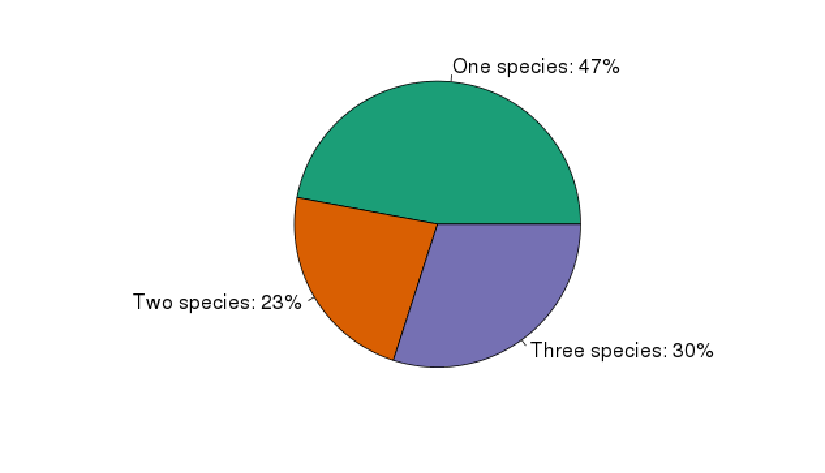
\includegraphics{fig5-14}
\caption{Proportions of all Dichaete-Dam binding intervals identified that are qualitatively conserved in one, two, and three species.}
\label{Figure 5.14}
\end{figure}

\emph{D. yakuba} has the highest percentage of unique binding intervals (32\%) and the lowest percentage of 3-way conserved binding intervals (42\%), while \emph{D. simulans} has the lowest percentage of unique binding intervals (15\%) and the highest percentage of 3-way conserved binding intervals (63\%). The correlation coefficients for read counts within all intervals between replicates within each species were quite high, ranging from 0.97 - 0.99 for \emph{D. melanogaster}, from 0.92 - 0.93 for \emph{D. simulans}, and from 0.96 - 0.98 for \emph{D. yakuba}. When comparing replicates between species, the correlations decrease to 0.65 - 0.74 between \emph{D. melanogaster} and \emph{D. simulans}, 0.69 - 0.71 between \emph{D. melanogaster} and \emph{D. yakuba}, and 0.64 - 0.72 between \emph{D. simulans} and \emph{D. yakuba} (Figure 5.15). Because of the greater variance between the \emph{D. simulans} replicates, it is difficult to determine whether Dichaete-Dam binding in \emph{D. melanogaster} is more similar to binding in \emph{D. simulans} or \emph{D. yakuba} based on the coefficients of correlations alone. To get a better idea of the overall similarities and differences between the different datasets, I also performed a principal component analysis (PCA) on all of the samples (Figure 5.16).\\

\begin{figure}
\centering
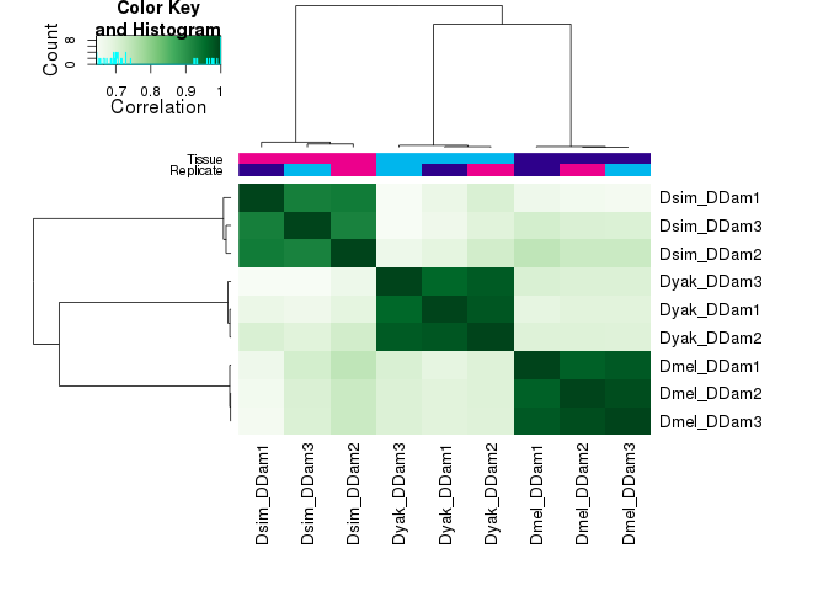
\includegraphics{fig5-15}
\caption{Clustering of \emph{D. melanogaster}, \emph{D. simulans} and \emph{D. yakuba} Dichaete-Dam samples by binding affinity scores in all bound intervals. Biological replicates from each species cluster strongly together. The color key and histogram shows the distribution of correlation coefficients for affinity scores in each pair of samples. Darker green corresponds to a higher correlation between samples, while lighter green corresponds to a lower correlation.}
\label{Figure 5.15}
\end{figure}

\begin{figure}
\centering
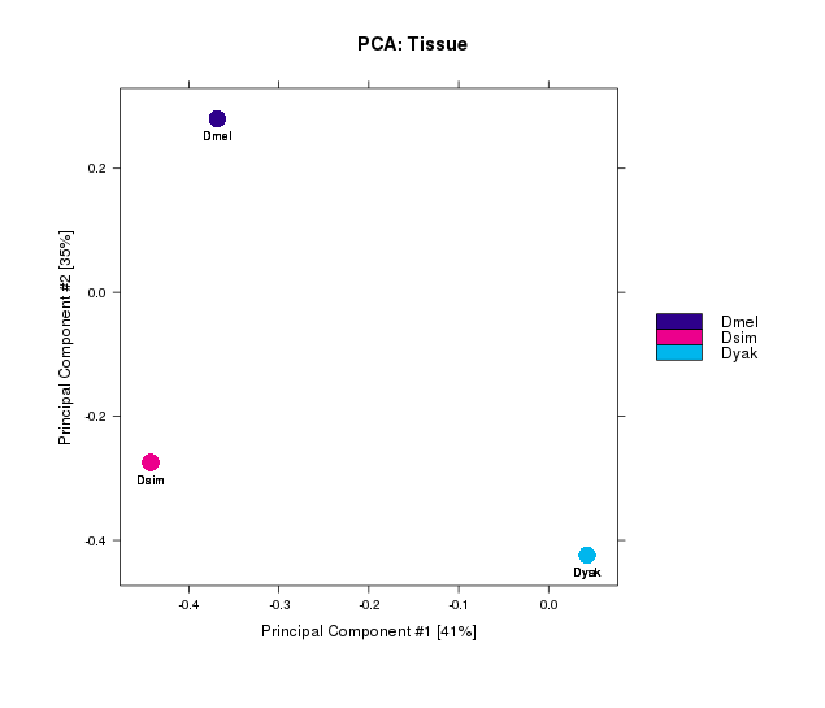
\includegraphics{fig5-16}
\caption{Prinicipal component analysis of binding affinity scores in bound intervals for \emph{D. melanogaster}, \emph{D. simulans} and \emph{D. yakuba} Dichaete-Dam samples. The first principal component separates \emph{D. yakuba} from the other two species, while the second principal component separates \emph{D. melanogaster} from \emph{D. simulans} and \emph{D. yakuba}.}
\label{Figure 5.16}
\end{figure}

The first principal component, which explains 41\% of the variation at bound intervals, separates \emph{D. melanogaster} and \emph{D. simulans} from \emph{D. yakuba}. The second principal component, which explains 35\% of the variation at bound intervals, separates \emph{D. melanogaster} from \emph{D. simulans} and \emph{D. yakuba}. This indicates that the primary driver of variation between the three species corresponds to changes in binding in \emph{D. yakuba} relative to the other two species, which is in line with the expectation of neutral evolution along the \emph{Drosophila} phylogeny, as \emph{D. yakuba} is the most distant from \emph{D. melanogaster} \citep{russo_molecular_1995}. In agreement with this observation, DiffBind identifies 5044 binding intervals that are differentially bound between \emph{D. melanogaster} and \emph{D. simulans} (Figure 5.17A), 8880 that are differentially bound between \emph{D. melanogaster} and \emph{D. yakuba} (Figure 5.17B), and 6324 that are differentially bound between \emph{D. simulans} and \emph{D. yakuba} (Figure 5.17C). Although these numbers are different from the numbers of differentially bound intervals detected in pairwise comparisons by DiffBind, since the pairwise comparisons started with different total sets of intervals and normalized the affinity scores between different sets of samples, the two analyses are broadly in agreement.\\

As with the pairwise comparisons, the percentages of all \emph{D. melanogaster} binding intervals that are identified as divergent in another species using a three-way comparison increase with phylogenetic distance. According to this analysis, 6.9\% of all \emph{D. melanogaster} intervals are qualitatively absent in \emph{D. simulans}, while 9.6\% are present but show quantitative changes in binding affinity. 11.6\% of \emph{D. melanogaster} intervals are qualitatively absent in \emph{D. yakuba}, while 20.4\% are present but show quantitative changes in binding affinity. The proportion of divergent intervals that are due to quantitative changes also increases with phylogenetic distance, from 58.0\% in \emph{D. simulans} to 63.7\% in \emph{D. yakuba}. By normalizing the data from all three species together, this three-way comparison presents a more generalized picture of how Dichaete binding varies both qualitatively and quantitatively across the melanogaster clade and confirms the phylogenetic patterns observed in pairwise comparisons.


\begin{figure}[H]
\centering
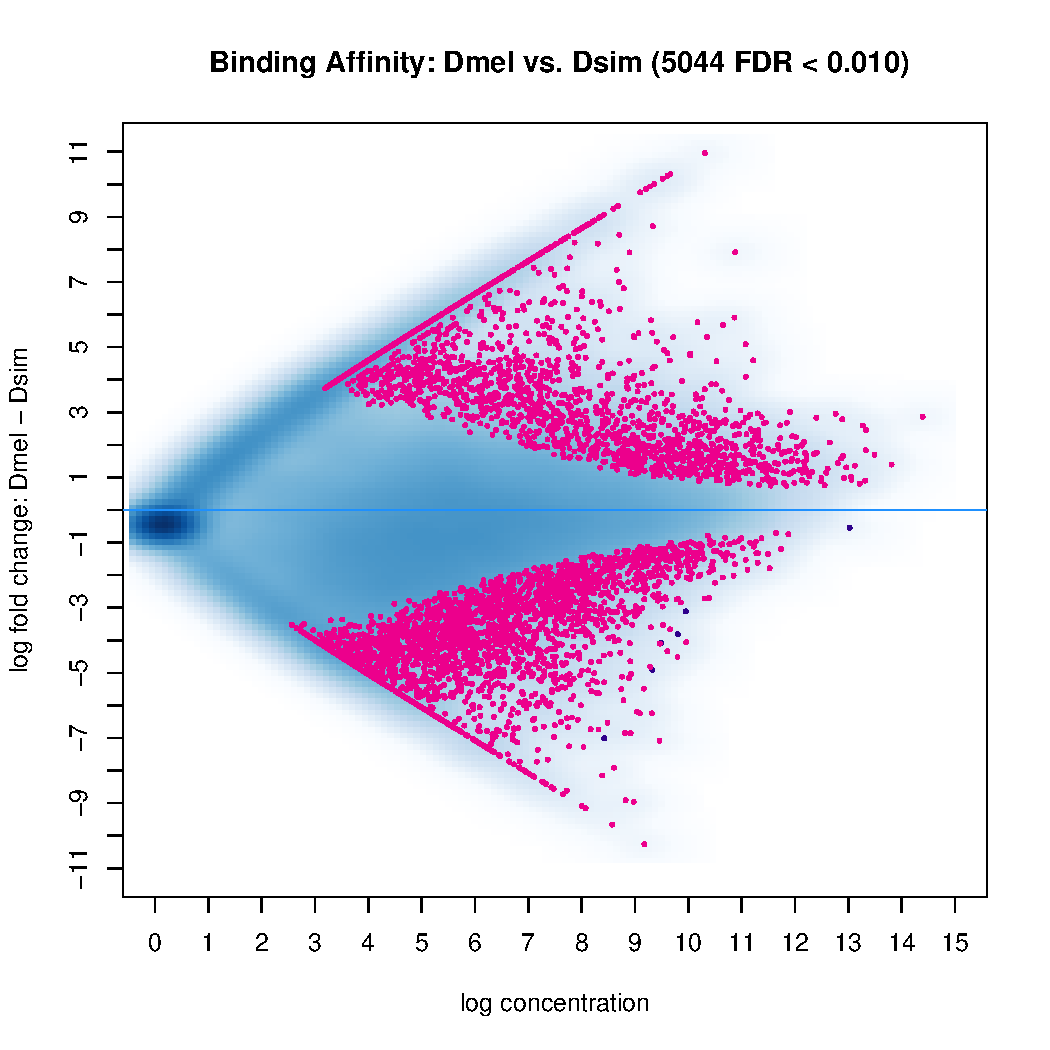
\includegraphics[width=10cm]{fig5-17a}
\label{Figure 5.17}
\end{figure}

\begin{figure}[H]
\centering
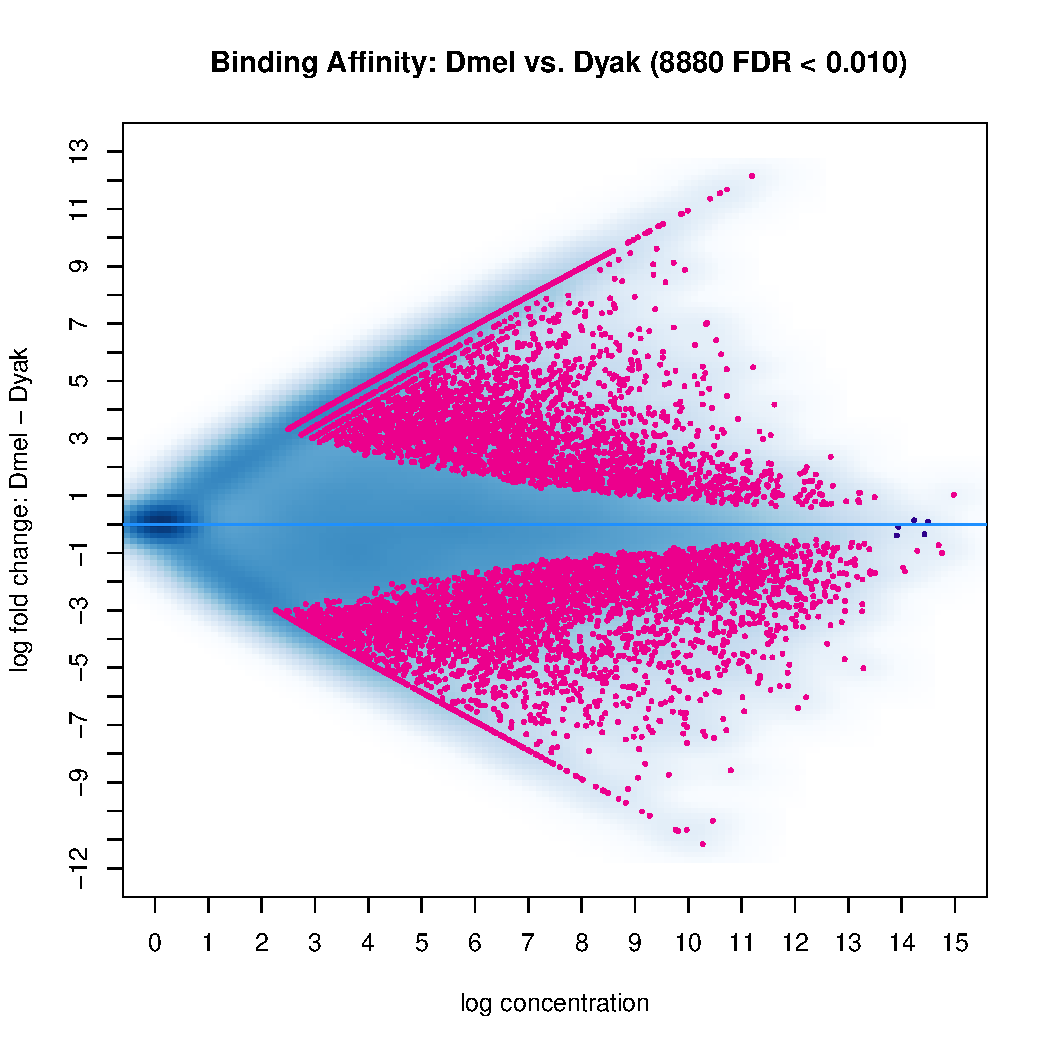
\includegraphics[width=10cm]{fig5-17b}
\label{Figure 5.17}
\end{figure}

\begin{figure}[H]
\centering
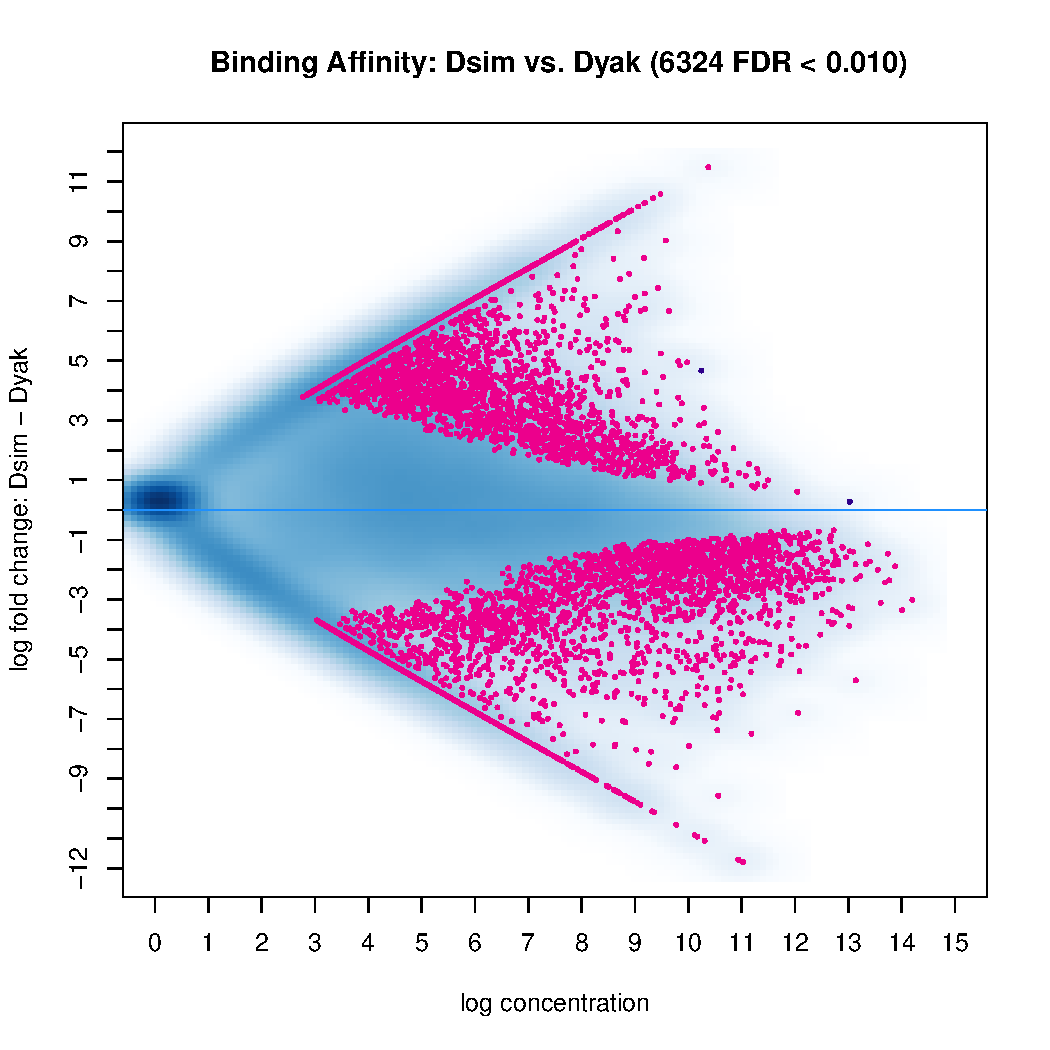
\includegraphics[width=10cm]{fig5-17c}
\caption{MA plots showing differentially bound Dichaete-Dam intervals with FDR \textless 0.01 between pairs of species using normalization between three species. A.) Differentially bound intervals between \emph{D. melanogaster} and \emph{D. simulans}. Intervals that are more strongly bound in \emph{D. melanogaster} have a positive log fold change, while intervals that are more strongly bound in \emph{D. simulans} have a negative log fold change. B.) Differentially bound intervals between \emph{D. melanogaster} and \emph{D. yakuba}. Intervals that are more strongly bound in \emph{D. melanogaster} have a positive fold change, while intervals that are differentially bound in \emph{D. yakuba} have a negative fold change. C.) Differentially bound intervals between \emph{D. simulans} and \emph{D. yakuba}. Intervals that are more strongly bound in \emph{D. simulans} have a positive fold change, while intervals that are more strongly bound in \emph{D. yakuba} have a negative fold change. All intervals are plotted; differentially bound intervals are highlighted in pink.}
\label{Figure 5.17}
\end{figure}


\section{Binding site turnover within gene loci}
It has been hypothesized that, as the percentage of conserved binding events at orthologous positions decreases between more distantly related species, new binding events at the same gene loci should evolve in order to maintain the same level of gene expression; this is often referred to as binding site turnover or compensatory evolution \cite{arnold_quantitative_2014,bradley_binding_2010,he_does_2011,moses_large-scale_2006}. In order to detect instances where a binding interval that is lost in one species might be compensated for by the gain of a new binding interval at the same gene locus in another species, I first took the set of all binding intervals called for each factor in each species, then did pairwise comparisons to find those intervals in one species that did not overlap with any binding intervals in the other. I did this for Dichaete-Dam between \emph{D. melanogaster} and \emph{D. simulans} and between \emph{D. melanogaster} and \emph{D. yakuba}, as well as for SoxN-Dam between \emph{D. melanogaster} and \emph{D. simulans}; I excluded \emph{D. pseudoobscura} because of the highly mismatched numbers of binding intervals called between it and \emph{D. melanogaster}. I then took the resulting lists of intervals and assigned them all to the nearest genes within 10 kb upstream or downstream, as described previously. Finally, I found every instance where two non-overlapping binding intervals, one from each species, were annotated to the same gene. I considered these intervals to show compensatory, rather than positional, conservation between each pair of species. An example of compensatory conservation at the \emph{reduced ocelli (rdo)} locus between \emph{D. melanogaster} and \emph{D. yakuba} is shown in Figure 5.18.\\ 

\begin{figure}
\centering
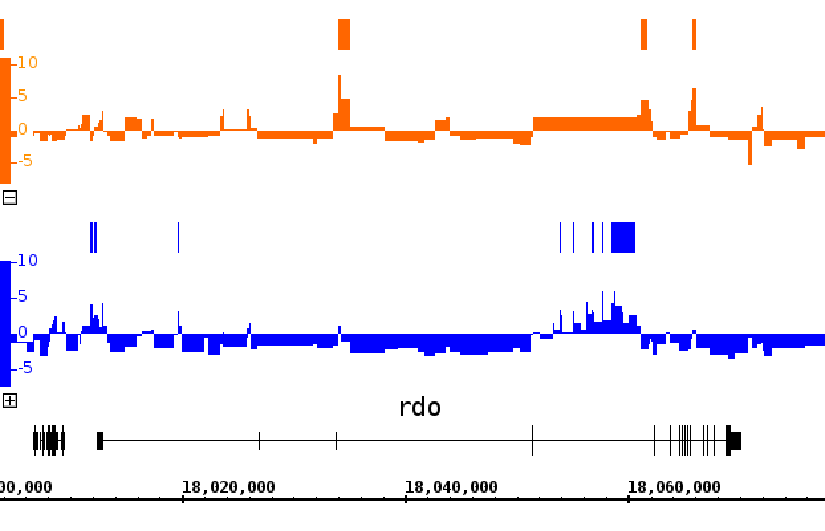
\includegraphics{fig5-18}
\caption{Dichaete-Dam binding site turnover between \emph{D. melanogaster} and \emph{D. yakuba} at the \emph{reduced ocelli (rdo)} locus. Tracks are, from bottom, gene models (black), \emph{D. melanogaster} Dichaete-Dam binding profile (blue), \emph{D. melanogaster} Dichaete-Dam FDR5 bound intervals (blue bars), \emph{D. yakuba} Dichaete-Dam binding profile (orange) and \emph{D. yakuba} Dichaete-Dam FDR5 bound intervals (orange bars). For clarity, bound intervals that are positionally conserved between both species are not shown. Strong binding is observed in the third, fourth and eleventh introns in \emph{D. yakuba}; these binding sites are lost in \emph{D. melanogaster}, but several binding intervals are gained in the first and fourth introns. Binding profiles represent normalized log2 ratios of Dichaete-Dam binding to Dam-only binding in each GATC fragment.}
\label{Figure 5.18}
\end{figure}

For Dichaete-Dam, I detected 5351 intervals in \emph{D. melanogaster} that show compensatory conservation relative to \emph{D. simulans}, and 3226 intervals in \emph{D. simulans} that show compensatory conservation relative to \emph{D. melanogaster}. In total, these pairs of intervals are located at 2457 unique genes. The greater number of compensatory intervals detected in \emph{D. melanogaster} may be due to the fact that more binding intervals were called in \emph{D. melanogaster} overall. I detected 4924 intervals for Dichaete-Dam in \emph{D. melanogaster} that show compensatory conservation relative to \emph{D. yakuba}, and 5083 that show compensatory conservation in \emph{D. yakuba} relative to \emph{D. melanogaster}, altogether located at 2806 unique genes. For SoxN-Dam, I detected 5497 binding intervals that show compensatory conservation in \emph{D. melanogaster} relative to \emph{D. simulans}, and 2939 that show compensatory conservation in \emph{D. simulans} relative to \emph{D. melanogaster}. These occur at 2393 unique genes.\\

Compensatory evolution has also been detected for active enhancers identified via STARR-seq; approximately 19\% of \emph{D. melanogaster} enhancers showed compensatory conservation in \emph{D. yakuba}, and this percentage increased with evolutionary distance, as the percentage of positionally conserved enhancers decreased \citep{arnold_quantitative_2014}. In the case of Dichaete-Dam, 23.6\% of \emph{D. melanogaster} binding intervals show compensatory conservation in \emph{D. yakuba}, a slightly higher rate than for STARR-seq enhancers. In order to determine whether turnover of binding intervals is correlated with turnover of active enhancers, I followed the same protocol to identify pairs of compensatory enhancers between \emph{D. melanogaster} and \emph{D. yakuba}. For both S2 and OSC STARR-seq enhancers, I found all enhancers in one species that do not overlap with any enhancer in the other; I then assigned these to the closest genes within 10kb upstream and downstream and found all instances where two non-overlapping enhancers from different species were annotated to the same gene. Starting with the unfiltered lists of STARR-seq enhancers, this resulted in 21105 S2 enhancers in \emph{D. melanogaster} that show compensatory conservation relative to \emph{D. yakuba} and 22444 in \emph{D. yakuba} that show compensatory conservation relative to \emph{D. melanogaster}. These pairs of enhancers are annotated to 7514 unique genes. For OSCs, it resulted in 17843 enhancers that show compensatory conservation in \emph{D. melanogaster} relative to \emph{D. yakuba} and 20207 in \emph{D. yakuba} that show compensatory conservation relative to \emph{D. melanogaster}. These pairs of enhancers are annotated to 6941 unique genes.\\

Of the Dichaete-Dam intervals that are compensatory in \emph{D. melanogaster} relative to \emph{D. yakuba}, 233 were previously annotated to a STARR-seq enhancer in S2 cells and 326 were annotated to a STARR-seq enhancer in OSCs. 53 of these S2 enhancers and 105 of these OSC enhancers also show compensatory conservation in \emph{D. melanogaster}. Conversely, of the Dichaete-Dam intervals that are compensatory in \emph{D. yakuba} relative to \emph{D. melanogaster}, 398 were previously annotated to a STARR-seq enhancer in S2 cells and 655 were annotated to a STARR-seq enhancer in OSCs. Only 90 of these S2 enhancers and 157 of these OSC enhancers also show compensatory conservation in \emph{D. yakuba}. This result was somewhat surprising, as I expected that the same forces driving turnover of enhancer function between the two species would also drive turnover of group B Sox binding. However, it shows that, while some instances of the evolution of a new, compensatory Dichaete binding site in one species are located within compensatory enhancers in that species, the majority of Dichaete binding turnover events happen either in active enhancers that are positionally conserved in both species or outside of annotated STARR-seq enhancers. Because Dichaete and SoxN show such strong overlap in binding and an ability to compensate for each other’s loss \citep{ferrero_soxneuro_2014}, it is possible that a SoxN binding site might evolve to compensate for the loss of a Dichaete binding site within some enhancers; unfortunately, I was unable to test this without in vivo SoxN binding data in \emph{D. yakuba}.\\
 
\section{Binding conservation and regulatory function}
\subsection{Binding conservation at known enhancers}
In my analysis of Dichaete-Dam and SoxN-Dam binding intervals in \emph{D. melanogaster}, I found a high rate of overlap between group B Sox binding and known enhancers from the REDFly and FlyLight databases \citep{gallo_redfly_2010,manning_resource_2012}. In order to test the hypothesis that conservation of binding between species should reflect functionality, I examined the proportion of binding intervals that are qualitatively conserved both within these known enhancers and outside of them. For Dichaete-Dam, I used the binding intervals identified in the three-way binding comparison in \emph{D. melanogaster, D. simulans}, and \emph{D. yakuba}. I considered three-way binding site conservation as well as pairwise conservation between \emph{D. melanogaster} and each other species. For SoxN-Dam, I used the binding intervals identified in the pairwise comparison between \emph{D. melanogaster} and \emph{D. simulans}. I compared the conservation status of binding intervals that overlap with known REDFly and FlyLight enhancers and those that do not.\\

While a relatively low number of Dichaete-Dam binding intervals overlap REDFly enhancers (751 total intervals), 64.4\% of these show three-way conservation between all species, compared to only 44.8\% of all binding intervals that do not overlap a REDFly enhancer (Figure 5.19A). Only 9.6\% of binding intervals overlapping a REDFly enhancer are unique to \emph{D. melanogaster}, while 27.6\% of those that do not overlap an enhancer are unique. Looking at pairwise conservation, being located within an enhancer does not have much of an effect; 3.6\% of intervals within a REDFly enhancer are conserved between \emph{D. melanogaster} and \emph{D. simulans} compared to 7.2\% of intervals that are not within an enhancer, while 22.2\% of intervals within a REDFly enhancer are conserved between \emph{D. melanogaster} and \emph{D. yakuba} compared to 20.3\% of intervals that are not within a REDFly enhancer. However, performing a chi-squared test on this data reveals that, overall, the difference in conservation between binding intervals that do or do not overlap a REDFly enhancer is highly significant (\(\chi\)\textsuperscript{2} = 161.9, d.f. = 3, p-value = 7.06e-35).\\

\begin{figure}
\centering
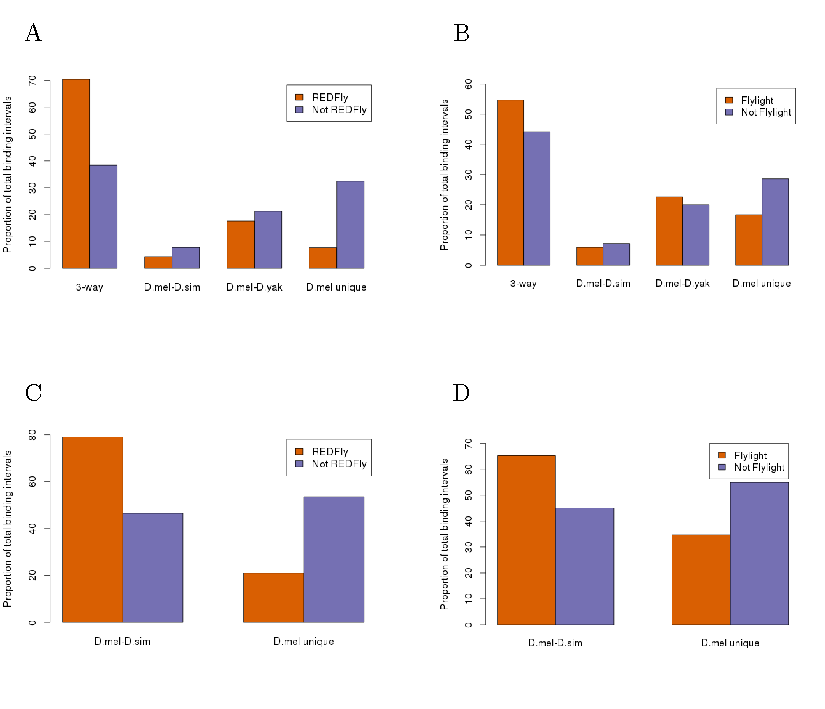
\includegraphics{fig5-19}
\caption{DamID binding intervals that overlap an annotated enhancer are more likely to be conserved than those that do not. A.) Dichaete-Dam binding intervals that overlap with a REDFly enhancer are more likely to show three-way conservation between \emph{D. melanogaster, D. simulans} and \emph{D. yakuba} (“3-way”) and are less likely to be unique to \emph{D. melanogaster}  (“D. mel unique”) than those that do not overlap with a REDFly enhancer (p \textless 2.2e-16).  B.) Dichaete-Dam binding intervals that overlap with a FlyLight enhancer are more likely to show three-way conservation between \emph{D. melanogaster, D. simulans} and \emph{D. yakuba} (“3-way”) and are less likely to be unique to \emph{D. melanogaster}  (“D. mel unique”) than those that do not overlap with a FlyLight enhancer (p \textless 2.2e-16). C.) SoxN-Dam binding intervals that overlap with a REDFly enhancer are more likely to be conserved between \emph{D. melanogaster} and \emph{D. simulans} (“D. mel - D. sim”) and less likely to be unique to \emph{D. melanogaster} (“D. mel unique”) than those that do not overlap with a REDFly enhancer (p \textless 2.2e-16). D.) SoxN-Dam binding intervals that overlap with a FlyLight enhancer are more likely to be conserved between \emph{D. melanogaster} and \emph{D. simulans} (“D. mel - D. sim”) and less likely to be unique to \emph{D. melanogaster} (“D. mel unique”) than those that do not overlap with a FlyLight enhancer (p = 7.27e-12).}
\label{Figure 5.19}
\end{figure}
 
A similar pattern can be seen with the FlyLight enhancers, although the effect is slightly smaller (Figure 5.19B). In this case, a total of 2531 Dichaete-Dam binding intervals overlap with an enhancer. 54.7\% of these intervals show three-way conservation between \emph{D. melanogaster, D. simulans} and \emph{D. yakuba}, compared to 44.2\% of binding intervals that do not overlap with an enhancer. 5.9\% of binding intervals located within a FlyLight enhancer show pairwise conservation between \emph{D. melanogaster} and \emph{D. simulans} compared to 7.2\% of intervals that are not located within an enhancer, while 22.6\% of binding intervals located within a FlyLight enhancer show pairwise conservation between \emph{D. melanogaster} and \emph{D. yakuba} compared to 20.0\% of intervals outside of an enhancer. Only 16.7\% of intervals overlapping a FlyLight enhancer are unique to \emph{D. melanogaster}, while 28.6\% of intervals not overlapping an enhancer are unique. Again, a chi-squared test shows that the effect of being located within a FlyLight enhancer on conservation is highly significant (\(\chi\)\textsuperscript{2} = 177.3, d.f. = 3, p-value = 3.38e-38).\\

For SoxN, a set of binding intervals with three-way conservation was not available; however, even at the level of two-way conservation between \emph{D. melanogaster} and \emph{D. simulans}, binding intervals that are located within known enhancers are much more likely to be conserved. The effect is particularly strong for REDFly enhancers. A total of 799 SoxN-Dam binding intervals are located within a REDFly enhancer; 79.0\% of these are qualitatively conserved between \emph{D. melanogaster} and \emph{D. simulans}, while only 46.5\% of binding intervals located outside of a REDFly enhancer are conserved. Conversely, 21.0\% of intervals within a REDFly enhancer are unique to \emph{D. melanogaster}, compared to 53.5\% of binding intervals not within a REDFly enhancer (Figure 5.19C). This effect is highly significant according to a chi-squared test (\(\chi\)\textsuperscript{2} = 323.6, d.f. = 1, p-value = 2.40e-72). The effect of being located within a FlyLight enhancer on conservation is slightly less strong but still substantial. 2844 SoxN-Dam binding intervals overlap a FlyLight enhancer; of these, 65.3\% are conserved between \emph{D. melanogaster} and \emph{D. simulans}, compared to 45.1\% of intervals outside of a FlyLight enhancer. 34.7\% of binding intervals within a FlyLight enhancer are unique to \emph{D. melanogaster}, while 54.9\% of those not within a FlyLight enhancer are unique (Figure 5.19D). Again, a chi-squared test shows that this is a significant effect (\(\chi\)\textsuperscript{2} = 46.95, df = 1, p-value = 7.27e-12). The strong increase in conservation observed for binding intervals within enhancers indicates that these binding sites are likely under balancing selection to maintain their effect on gene regulation and confirms the hypothesis that functionally important binding events should show a high rate of evolutionary conservation.

\subsection{Binding conservation at group B Sox core intervals}
I was also interested in testing whether the core Dichaete and SoxN binding intervals that were previously identified in \emph{D. melanogaster} were highly conserved between species. Since these intervals were identified in multiple experiments, we have high confidence that they are functional in the sense that they are truly bound \emph{in vivo} in \emph{D. melanogaster}; however, they are not necessarily the sites of direct gene regulatory activity by Dichaete and SoxN. Interestingly, I found that the FDR1 Dichaete-Dam binding intervals in \emph{D. melanogaster} showed a much greater overlap with Dichaete core intervals than the FDR1 SoxN-Dam binding intervals did with SoxN core intervals.\\

Of the binding intervals identified in the three-way comparison for Dichaete-Dam, a total of 3855 overlap a Dichaete core interval. Of these, 70.4\% show three-way conservation between \emph{D. melanogaster, D. simulans} and \emph{D. yakuba}, while only 38.5\% of binding intervals that do not overlap a Dichaete core interval show three-way conservation (Figure 5.20A). Only 7.7\% of binding intervals that overlap a Dichaete core interval are unique to \emph{D. melanogaster}, compared to 32.4\% of binding intervals that do not overlap a core interval. Somewhat surprisingly, binding intervals that overlap core intervals are not more likely to show two-way conservation; 4.3\% show conservation between \emph{D. melanogaster} and \emph{D. simulans} compared to 7.8\% of binding intervals that do not overlap a core interval, and 17.6\% show conservation between \emph{D. melanogaster} and \emph{D. yakuba} compared to 21.2\% of binding intervals that do not overlap a core interval. Nonetheless, the effect of overlapping a core Dichaete binding interval on the pattern of conservation is highly significant according to a chi-squared test (\(\chi\)\textsuperscript{2} = 1408.6, d.f. = 3, p-value = 4.10-305).\\

\begin{figure}
\centering
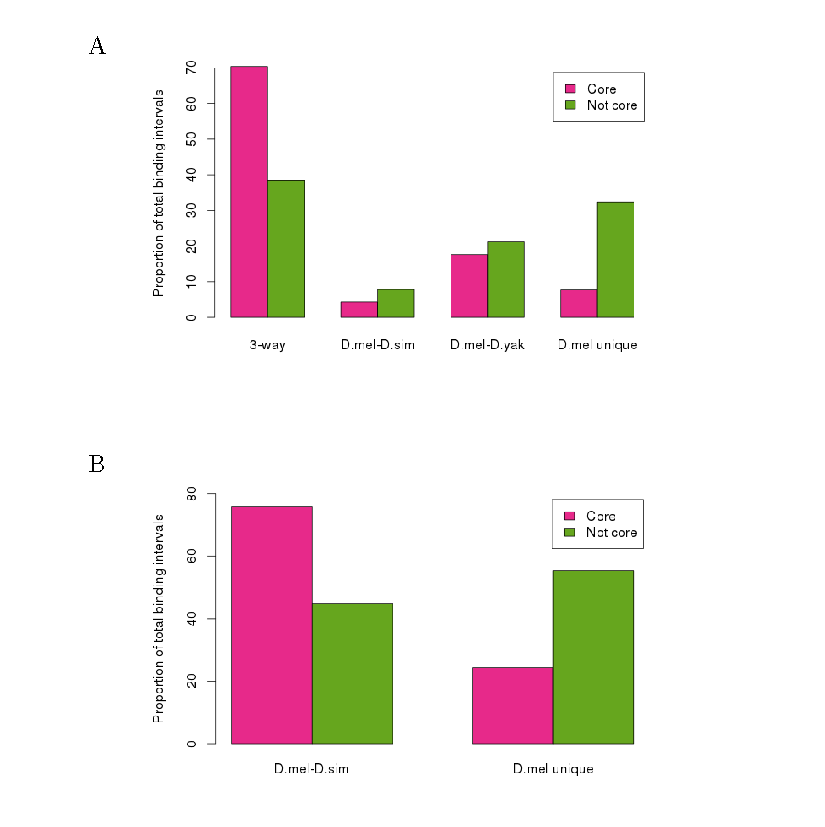
\includegraphics{fig5-20}
\caption{DamID binding intervals that overlap a Dichaete or SoxN core binding interval are more likely to be conserved than those that do not. A.) Dichaete-Dam binding intervals that overlap with a core Dichaete interval are more likely to show three-way conservation between \emph{D. melanogaster, D. simulans} and \emph{D. yakuba} (“3-way”) and are less likely to be unique to \emph{D. melanogaster}  (“D. mel unique”) than those that do not overlap with a core interval (p \textless 2.2e-16). B.) SoxN-Dam binding intervals that overlap with a core SoxN interval are more likely to be conserved between \emph{D. melanogaster} and \emph{D. simulans} (“D. mel - D. sim”) and less likely to be unique to \emph{D. melanogaster} (“D. mel unique”) than those that do not overlap with a core interval (p \textless 2.2e-16).}
\label{Figure 5.20}
\end{figure}

In the case of SoxN-Dam, a total of 2111 binding intervals overlap a SoxN core interval. Of these, 75.7\% show two-way conservation between \emph{D. melanogaster} and \emph{D. simulans}, while 44.7\% of binding intervals that do not overlap SoxN core interval show conservation (Figure 5.20B). Conversely, only 24.3\% of binding intervals that overlap a core interval are unique to \emph{D. melanogaster}, compared to 55.3\% of binding intervals that do not overlap a core interval. Again, this effect is highly significant according to a chi-squared test (\(\chi\)\textsuperscript(2) = 733.1, d.f. = 1, p-value = 1.90e-161).\\  

These results suggest that binding events at the Dichaete and SoxN core intervals, although they may not all represent direct gene regulation events, are nonetheless functionally important and subject to evolutionary constraint. It is somewhat surprising that, in the case of the core intervals as well as known enhancers, a strong effect on conservation between \emph{D. melanogaster} and \emph{D. simulans} is observed for SoxN, but this effect is missing for Dichaete. In contrast, for Dichaete, a strong effect is only observed on three-way binding conservation, with a smaller effect being observed for conservation between \emph{D. melanogaster} and \emph{D. yakuba} in the case of known enhancers. This may be because, over the relatively short evolutionary distance between \emph{D. melanogaster} and \emph{D. yakuba}, the majority of the binding events that are under selective pressure have been conserved between all three species, whereas few binding events are selectively constrained in only two out of the three lineages. For SoxN, where only data from two species are available, the conserved binding events likely also encompass many binding intervals that would be conserved in \emph{D. yakuba} as well. Unfortunately, it is not possible to directly test this hypothesis with the current datasets.

\subsection{Binding conservation at Dichaete and SoxN direct targets}
A list of genes that are direct targets of both Dichaete and SoxN has previously been compiled by integrating gene expression data and in vivo binding data \citep{aleksic_role_2013,ferrero_soxneuro_2014}. I expected binding events at these genes to be highly conserved as well, since they are functional targets in \emph{D. melanogaster}. For Dichaete-Dam, of the total binding intervals identified in a three-way comparison between \emph{D. melanogaster, D. simulans} and \emph{D. yakuba}, 4301 are annotated to a Dichaete direct target gene. This includes instances where multiple intervals are annotated to the same gene. 53.7\% of these are conserved in all three species, compared to 43.1\% of intervals that are not annotated to a direct target gene (Figure 5.21A). There is very little difference in the rates of two-way conservation between intervals annotated to direct targets and those that are not. Of the intervals at direct target genes, 20.4\% are unique to \emph{D. melanogaster}, compared to 29.0\% of intervals not at direct target genes. Although these differences are significant according to a chi-squared test (\(\chi\)\textsuperscript{2} = 57.3, d.f. = 3, p-value = 2.3e-12), the effect on conservation rates is smaller than for binding intervals that overlap a core Dichaete interval.\\

\begin{figure}
\centering
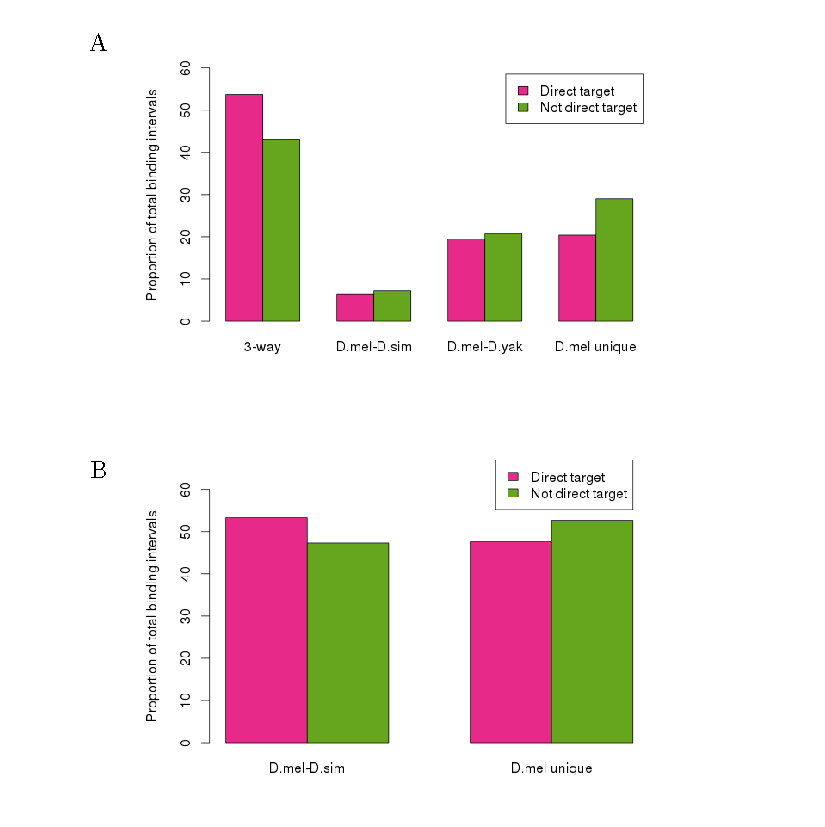
\includegraphics{fig5-21}
\caption{DamID binding intervals that are annotated to a Dichaete or SoxN direct target gene are more likely to be conserved that those that are not. A.) Dichaete-Dam binding intervals that are annotated to a Dichaete direct target gene are more likely to show three-way conservation between \emph{D. melanogaster}, \emph{D. simulans} and \emph{D. yakuba} (“3-way”) and are less likely to be unique to \emph{D. melanogaster} (“D. mel unique”) than those that are not annotated to a direct target (p = 2.3e-12). B.) SoxN-Dam binding intervals that are annotated to a SoxN direct target gene are more likely to be conserved between \emph{D. melanogaster} and \emph{D. simulans} (“D. mel - D. sim”) and less likely to be unique to \emph{D. melanogaster} (“D. mel unique”) than those that are not annotated to a direct target (p = 3.4e-05).}
\label{Figure 5.21}
\end{figure}

In the case of SoxN-Dam, there is even less of an effect. Of the total SoxN-Dam binding intervals identified in a comparison between \emph{D. melanogaster} and \emph{D. simulans}, 1849 are annotated to a SoxN direct target gene. The fact that less binding intervals are located at direct targets is likely because less direct target genes have been identified for SoxN than for Dichaete. Of these, 53.3\% are conserved between the two species, compared to 47.3\% of binding intervals that are not annotated to a direct target (Figure 5.21B). Conversely, 47.6\% of intervals annotated to direct targets are unique to \emph{D. melanogaster}, while 52.7\% of intervals not annotated to direct targets are unique to that species. These differences are significant according to a chi-squared test (\(\chi\)\textsuperscript{2} = 17.2, d.f. = 1, p-value = 3.4e-05). Initially, it was somewhat surprising to see that binding intervals at direct target genes are less likely to be conserved than those at core intervals, since binding at direct targets should be functional by definition. However, in many cases multiple intervals are annotated to a single target gene. Some of these binding events may be less important for gene regulation than others, perhaps representing shadow enhancers, and may therefore be less constrained by natural selection \citep{ludwig_consequences_2011,perry_shadow_2010}. The presence of these binding intervals in the dataset under consideration likely reduces the overall rate of conservation of intervals annotated to direct target genes.

\section{Evolutionary perspective on common and unique binding by Dichaete and SoxNeuro}
As was briefly discussed in the previous chapter, there are differences in the relationship between Dichaete-Dam and SoxN-Dam binding in \emph{D. melanogaster} and \emph{D. simulans}; most obviously, Dichaete-Dam and SoxN-Dam show considerably higher overlap in their binding patterns in \emph{D. melanogaster}. I wanted to understand these differences better by examining the relationship between common and unique binding by Dichaete and SoxN and binding conservation. On a qualitative level, 15900 binding intervals are common to Dichaete and SoxN in \emph{D. melanogaster}, while 9114 are common to Dichaete and SoxN in \emph{D. simulans}; 7415 of these are commonly bound in both species, representing 46.7\% of commonly bound intervals in \emph{D. melanogaster} and 81.4\% of commonly bound intervals in \emph{D. simulans} (Figure 5.22). In \emph{D. melanogaster}, 2634 binding intervals are unique to Dichaete-Dam, while in \emph{D. simulans}, 4293 are unique to Dichaete-Dam. Only 338 of these are present and uniquely bound in both species, representing a much lower rate of conservation. The case is similar for SoxN-Dam; out of 4079 uniquely-bound intervals in \emph{D. melanogaster} and 3741 uniquely-bound intervals in \emph{D. simulans}, only 300 are present and uniquely bound in the two species. This suggests that binding intervals where both Dichaete and SoxN bind may be under greater evolutionary constraint than intervals where only one of the two proteins binds. Additionally, there are considerably more intervals that are uniquely bound by either protein in \emph{D. simulans} and are commonly bound in \emph{D. melanogaster} than the inverse (3372 versus 750), supporting the observation that Dichaete and SoxN binding patterns appear to be more differentiated in \emph{D. simulans} than in \emph{D. melanogaster}.\\

\begin{figure}
\centering
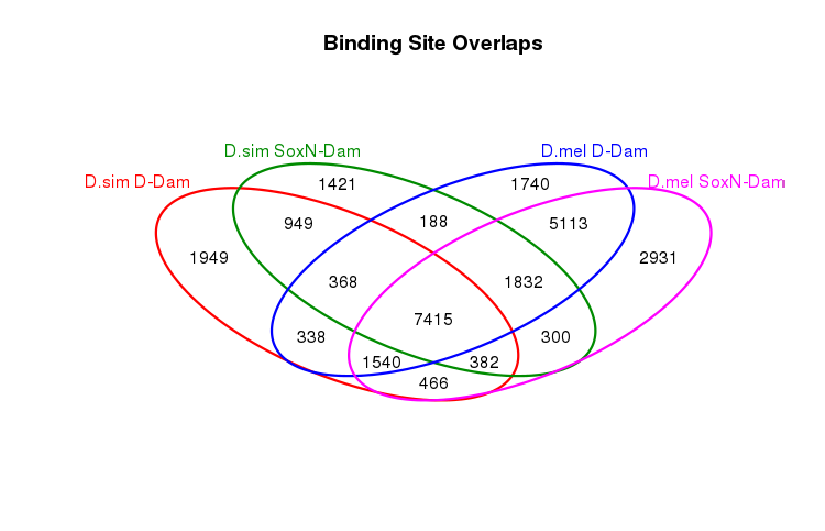
\includegraphics[trim=0cm 1cm 0cm 2cm, clip]{fig5-22}
\caption{Venn diagram showing overlaps between Dichaete-Dam and SoxN-Dam binding intervals in \emph{D. melanogaster} and \emph{D. simulans}. A greater proportion of conserved intervals are uniquely bound by either Dichaete or SoxN in \emph{D. simulans} but commonly bound by both TFs in \emph{D. melanogaster} than the reverse.}
\label{Figure 5.22}
\end{figure}

Taking just the binding intervals identified in \emph{D. melanogaster}, there is a clear association between common binding by Dichaete and SoxN and binding conservation. 76.5\% of binding intervals that are commonly bound are conserved in \emph{D. simulans}, while 23.5\% of them are not. In contrast, 40.1\% of intervals that are uniquely bound by Dichaete are conserved in \emph{D. simulans}, while 59.9\% are not, and only 33.7\% of intervals that are uniquely bound by SoxN are conserved in \emph{D. simulans}, while 66.3\% are not (Figure 5.23A). The difference in conservation between commonly and uniquely bound intervals is highly significant according to a chi-squared test (\(\chi\)\textsuperscript{2} = 3398.3, d.f. = 2, p-value \textless 2.2e-16 [approaches 0]). When the same analysis is performed from the perspective of binding intervals identified in \emph{D. simulans}, a striking amount of intervals that are commonly bound by Dichaete and SoxN, 94.1\%, are conserved in \emph{D. melanogaster}, while just 5.9\% are unique to \emph{D. simulans} (Figure 5.23B). Unlike the \emph{D. melanogaster} intervals, while the uniquely bound intervals in \emph{D. simulans} show less conservation than the commonly bound intervals, they are still more likely to be conserved than not. 62.8\% of intervals that are uniquely bound by Dichaete are conserved in \emph{D. melanogaster}, while 37.2\% are not, and 70.1\% of intervals that are uniquely bound by SoxN are conserved in \emph{D. melanogaster}, while 29.9\% are not. However, the overall difference in conservation rates between commonly and uniquely bound intervals is still highly significant (\(\chi\)\textsuperscript{2} = 2488.9, d.f. = 2, p-value \textless 2.2e-16 [approaches 0]).\\

\begin{figure}
\centering
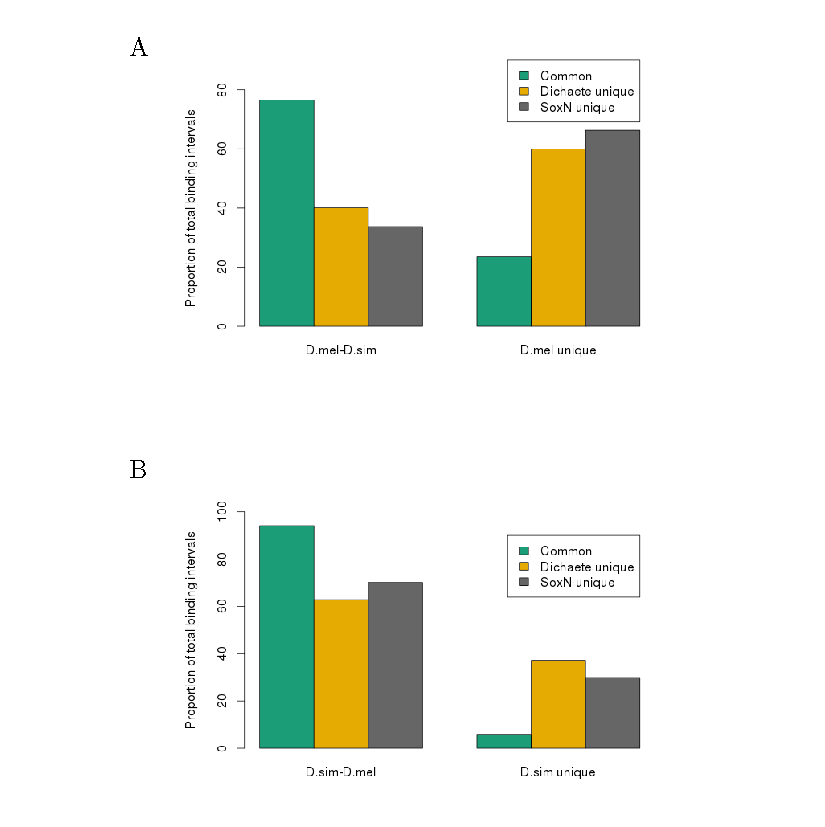
\includegraphics{fig5-23-1}
\caption{Intervals that are commonly bound between Dichaete-Dam and SoxN-Dam are more likely to be conserved between \emph{D. melanogaster} and \emph{D. simulans} than intervals that are uniquely bound by either Dichaete-Dam or SoxN-Dam. A.) Of all \emph{D. melanogaster} binding intervals, those that are bound by both Dichaete-Dam and SoxN-Dam (“Common”) are more likely to also be bound in \emph{D. simulans} (“D. mel - D. sim”) and less likely to be unique to \emph{D. melanogaster} (“D. mel unique”) than those that are uniquely bound by either Dichaete-Dam or SoxN-Dam (p \textless 2.2e-16). B.) Of all \emph{D. simulans} binding intervals, those that are bound by both Dichaete-Dam and SoxN-Dam (“Common”) are more likely to also be bound in \emph{D. melanogaster} (“D. sim - D. mel”) and less likely to be unique to \emph{D. simulans} (“D. sim unique”) than those that are uniquely bound by either Dichaete-Dam or SoxN-Dam (p \textless 2.2e-16).}
\label{Figure 5.23}
\end{figure}

Assigning these conserved, commonly bound intervals to the closest genes within 10 kb upstream or downstream results in the identification of 5966 conserved core group B Sox targets in \emph{D. melanogaster} and \emph{D. simulans} (Appendix X). These gene targets have a profile that is consistent with the classical picture of group B Sox function. They are primarily upregulated in the larval CNS according to FlyAtlas, and they are enriched for GO:BP terms related to biological regulation (p = 1.48e-49), system development (p=2.86e-37), anatomical structure morphogenesis (p=6.41e-32), generation of neurons (p=4.55e-31) and neuron differentiation (p=4.92e-28) (Appendix X). To examine the evolutionary conservation of these target genes on an expanded scale, I compared them with targets of Sox2, Sox3 and Sox11, a group C Sox protein, identified in the mouse. I mapped the lists of bound genes discovered by Bergsland et al. to their \emph{D. melanogaster} orthologues, resulting in 1301 orthologous targets of Sox2 in mouse neural precursor cells (NPCs), 4213 orthologous targets of Sox3 in NPCs and 1485 orthologous targets of Sox11 in NPCs \citep{bergsland_sequentially_2011}. 589 of the Sox2 target orthologues, 1730 of the Sox3 target orthologues and 595 Sox11 orthologues are conserved and commonly bound by Dichaete and SoxN. These deeply conserved Sox target genes represent around 40-45\% of the targets of each mouse Sox protein but a smaller fraction of the commonly bound Dichaete/SoxN targets, indicating that, while Dichaete and SoxN can both perform aspects of mammalian Sox group B and C function, they have also both acquired a considerably broader range of targets in flies. A previous study of shared targets of Sox2 and Dichaete or SoxN core targets, as well as shared targets of Sox11 and SoxN, found similar numbers of orthologous target genes shared between Sox2 and each fly Sox protein individually. However, roughly twice as many targets were found to be shared between Sox11 and SoxN alone as between Sox11 and common Dichaete/SoxN targets, suggesting that while both Dichaete and SoxN may equally contribute to homologous functions of mammalian group B1 genes, Sox11’s role may be largely played by SoxN in the fly, rather than by both TFs \citep{ferrero_soxneuro_2014}. Overall, there is a high overlap between targets of mouse Sox genes from both groups B and C and common, conserved targets of Dichaete and SoxN in the fly, supporting the deep evolutionary conservation of Sox function in the CNS (Table 5.2).\\

\begin{table}[h]
\centering
\begin{tabular}{|p{2.3cm}|p{2.7cm}|p{3.0cm}|p{2.4cm}|p{2.4cm}|}
\hline
\textbf{Mouse Sox protein} & \textbf{Orthologues of mouse targets in \emph{D. melanogaster}} & \textbf{Overlap with Dichaete/SoxN common targets} & \textbf{Overlap with core SoxN targets} & \textbf{Overlap with core Dichaete targets} \\ \hline
Sox2              & 1301                                            & 589                                       & 443                            & 522                                \\ \hline
Sox3              & 4213                                            & 1730                                      & 1134                           & 1590                               \\ \hline
Sox11             & 1485                                            & 595                                       & 1092                           & 610                                \\ \hline
\end{tabular}
\caption{Numbers of shared target genes between \emph{Drosophila} orthologues of mouse group B and C Sox proteins and either common Dichaete/SoxN targets or core targets of Dichaete or SoxN in \emph{D. melanogaster}.}
\label{Table 5.2}
\end{table}

To examine the differential functions of Dichaete and SoxN in \emph{D. melanogaster} and \emph{D. simulans}, I assigned the lists of binding intervals that are uniquely bound by either Dichaete or SoxN in both species to the nearest \emph{D. melanogaster} genes within 10 kb upstream or downstream. This resulted in 381 gene assignments for Dichaete and 361 gene assignments for SoxN (Appendix X). Only 14 genes are shared between the two lists, meaning that, at the loci where Dichaete and SoxN bind uniquely in both species, they are largely regulating separate sets of genes. I used FlyMine to analyze the functional enrichments of these gene sets. The two sets of genes have clearly different spatial expression profiles according to the FlyAtlas gene expression data; the genes uniquely bound by SoxN are predominantly upregulated only in the larval CNS, while the genes uniquely bound by Dichaete are also upregulated in the larval hindgut, head, crop, brain and thoracicoabdominal ganglion. These results agree with the observed expression patterns of the unique targets of Dichaete-Dam and SoxN-Dam uncovered in both \emph{D. melanogaster} and \emph{D. simulans} by the single-species DiffBind analysis in Chapter 4. The two sets of genes have similar GO:BP enrichments, including terms related to morphogenesis, development, neuron differentiation and biological regulation (Appendix X). These results suggest that a primary difference between Dichaete and SoxN function may be that, while Dichaete and SoxN are involved in many similar functions during development, Dichaete has targets that are spatially expressed in a broader range of tissues, while the targets that are unique to SoxN are more limited to the developing CNS. Interestingly, the \emph{Drosophila} orthologues of mouse Sox11 targets, which overlap with more SoxN targets than common Dichaete/SoxN targets, are also primarily upregulated in the CNS, as opposed to orthologues of Sox2 targets, which also show upregulation in the brain.\\

I also searched for \emph{de novo} motifs in the intervals that are uniquely bound by both Dichaete and SoxN in both species in order to identify any potential co-regulators that might shape the unique functions of each TF. Several motifs corresponding to transcriptional regulators that play broad roles during development were identified in both sets of intervals, including DNA replication-related element factor (Dref, p=1e-8) and Tramtrack (Ttk, p=1e-6). One of the top motifs identified in the unique SoxN intervals corresponds to Ultraspiracle (Usp, p=1e-10), a TF involved in several aspects of neuron morphogenesis \citep{lee_cell-autonomous_????,parrish_genome-wide_2006}. Interestingly, one of the top hits in the unique Dichaete intervals is a Brachyenteron (Byn) motif (p=1e-9). Byn is a transcription factor that is critical for the development of the hindgut \citep{kispert_homologs_1994,murakami_developmental_1999}. The presence of this motif supports the idea that one of the primary unique functions of Dichaete, which is conserved in \emph{D. melanogaster} and \emph{D. simulans}, is its role regulating hindgut development.\\

I used DiffBind again to get a picture of the quantitative differences in Dichaete and SoxN binding in \emph{D. melanogaster} and \emph{D. simulans}. An analysis of differential binding between the two TFs using samples from both species with species as a blocking factor reveals 1257 binding intervals that are differentially bound at FDR1, with 778 of these preferentially bound by Dichaete-Dam and 479 preferentially bound by SoxN-Dam (Figure 5.24). Of the intervals preferentially bound by Dichaete-Dam, 681 were called as bound by Dichaete in both species in a single-species analysis. All of the intervals preferentially bound by SoxN-Dam were called as bound in both species in a single-species analysis. I assigned these differentially bound intervals to the nearest genes within 10 kb upstream and downstream in the \emph{D. melanogaster} genome. This resulted in 925 gene assignments for Dichaete-Dam and 526 for SoxN-Dam. 54 genes are annotated as targets in both datasets. Similar differences in spatial expression are observed among these sets of target genes as among the genes identified in the qualitative analysis of differential binding; Dichaete-Dam preferential targets are upregulated in a wider range of tissues including the brain, head, larval CNS, crop, adult eye, hindgut, and thoracicoabdominal ganglion, while SoxN-Dam preferential targets are strongly upregulated only in the larval CNS. The set of SoxN-Dam preferential targets is enriched for homeodomain proteins, which is not observed in the Dichaete-Dam preferential targets. Again, the top enriched GO:BP terms for the two sets of genes are quite similar. However, in this case the list of publications that are enriched for preferential SoxN-Dam targets contains some interesting hints as to their functions; several publications related to neural stem cell differentiation, self-renewal and transcriptional networks are top hits (p \textless 1e-21). There is also an enrichment of SoxN-Dam preferential target genes in the Reactome pathway “Role of Abl in Robo-Slit signalling”, an important pathway in axon guidance.\\

\begin{figure}
\centering
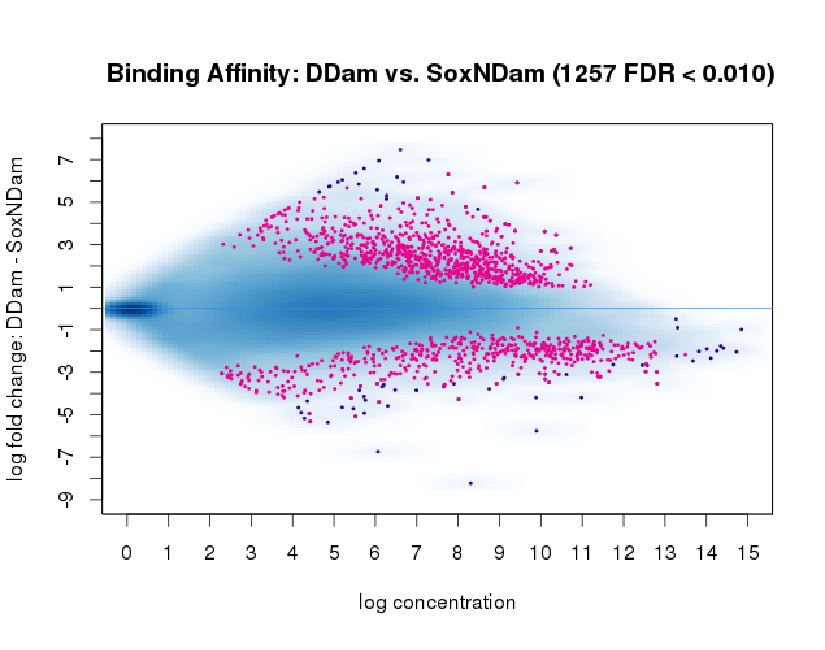
\includegraphics{fig5-24}
\caption{MA plot of differentially bound intervals with FDR \textless 0.01 between Dichaete-Dam and SoxN-Dam in both \emph{D. melanogaster} and \emph{D. simulans}, with species as a blocking factor. Intervals that are more strongly bound by Dichaete-Dam have a positive fold change, while intervals that are more strongly bound by SoxN-Dam have a negative fold change. All intervals are plotted; differentially bound intervals are highlighted in pink.}
\label{Figure 5.24}
\end{figure}

I expected that, in cases where a TF bound preferentially in one species, it also bound preferentially in the other species; however, I wondered if there were certain binding intervals where the opposite was the case. In order to address this, I compared the binding intervals that were preferentially bound by either Dichaete-Dam or SoxN-Dam in each species separately. Of all of the intervals preferentially bound by either TF in \emph{D. melanogaster} and \emph{D. simulans}, only 347 overlap in the two species. Plotting the log2 fold changes for Dichaete-Dam binding versus SoxN-Dam binding at these intervals in both species reveals an interesting pattern (Figure 5.25A). The majority of the intervals shared between the two species are preferentially bound by Dichaete-Dam (fold change \textgreater 0) in both species. A much smaller number are preferentially bound by SoxN-Dam (fold change \textless 0) in both species. Surprisingly, a similar number to those bound by SoxN-Dam are preferentially bound by Dichaete-Dam in one species and SoxN-Dam in the other, or vice versa. A linear regression of the fold changes in \emph{D. simulans} versus \emph{D. melanogaster} yields a positive but weak correlation of 0.19; this correlation is highly significant (p = 8.37e-18).\\

It is possible that the binding intervals with fold changes in the opposite direction in the two species represent extreme cases of Dichaete and SoxN’s ability to compensate for each other, to the extent that they have effectively swapped binding functions during evolution. I decided to investigate these binding intervals in more detail. There are 15 intervals that are bound more strongly by Dichaete-Dam in \emph{D. melanogaster} and more strongly by SoxN-Dam in \emph{D. simulans}, and there are 27 that are bound more strongly by Dichaete-Dam in \emph{D. simulans} and more strongly by SoxN-Dam in \emph{D. melanogaster}. I annotated these intervals to the closest genes within 10 kb upstream and downstream in the \emph{D. melanogaster} genome. Interestingly, some of them are annotated to known target genes with key roles in the developmental functions of Dichaete and SoxN. For example, a binding interval downstream of \emph{tll}, a target of Dichaete in the hindgut, is more strongly bound by Dichaete in \emph{D. melanogaster} but more strongly bound by SoxN in \emph{D. simulans} (Figure 5.25B). In the opposite scenario, binding intervals located in an intron of \emph{beat-IIa} (Figure 5.25C), also involved in axon guidance, and \emph{hth} (Figure 5.25D), a Ubx cofactor that is important for many aspects of body patterning during development, are more strongly bound by Dichaete in \emph{D. simulans} but more strongly bound by SoxN in \emph{D. melanogaster}. However, the differences in binding strength between Dichaete and SoxN at these intervals is largely quantitative rather than qualitative, and they also tend to be located within or near genes that have other, additional binding intervals, making it unclear whether the differences observed are of functional significance in gene regulation.\\

\begin{figure}[H]
\centering
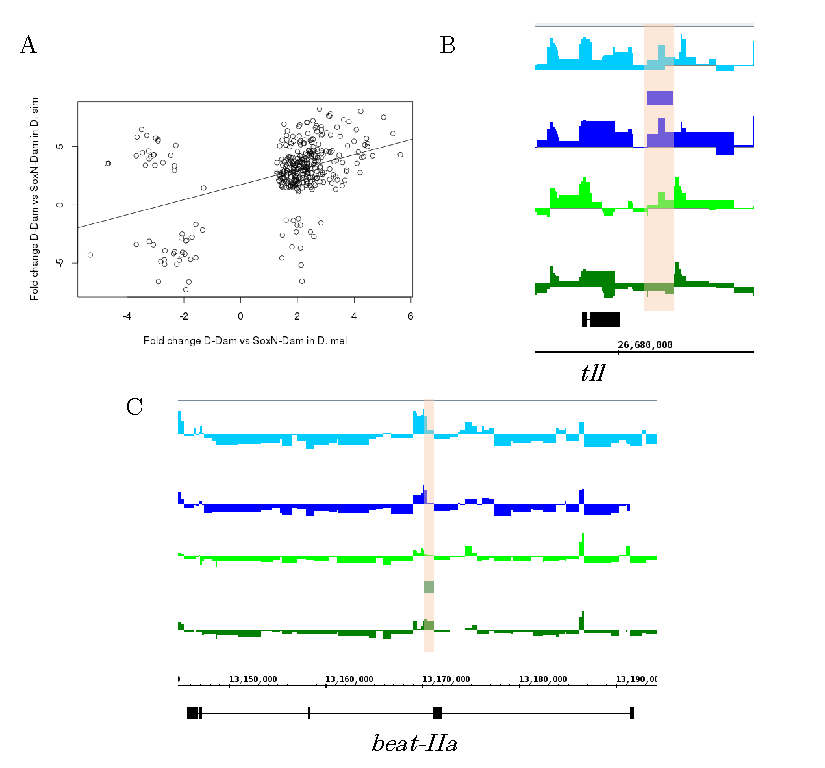
\includegraphics{fig5-25}
\caption{Differential binding between Dichaete-Dam and SoxN-Dam in \emph{D. melanogaster} versus in \emph{D. simulans}. A.) Scatter plot of fold changes between Dichaete-Dam and SoxN-Dam at differentially bound intervals in \emph{D. melanogaster} versus fold changes at orthologous, differentially bound intervals in \emph{D. simulans}. Positive fold changes indicate preferential binding by Dichaete-Dam in an interval, while negative fold changes indicate preferential binding by SoxN-Dam in an interval. The majority of intervals that are differentially bound in both species are preferentially bound by Dichaete-Dam in both species. Smaller numbers are preferentially bound by SoxN-Dam in both species or preferentially bound by Dichaete-Dam in one species and SoxN-Dam in the other (R\textsuperscript{2} = 0.19, p \textless 2.2e-16). B.) A binding interval downstream of \emph{tll} that is preferentially bound by Dichaete-Dam in \emph{D. melanogaster} (dark blue) but preferentially bound by SoxN-Dam in \emph{D. simulans} (light green). Binding profiles represent normalized log2 ratios of Dam-fusion protein binding to Dam-only binding in each GATC fragment. Tracks are, from the bottom, \emph{D. simulans} Dichaete-Dam in dark green, \emph{D. simulans} SoxN-Dam in light green, \emph{D. melanogaster} Dichaete-Dam in dark blue and \emph{D. melanogaster} SoxN-Dam in light blue. Dichaete-Dam binding intervals are represented by blue or green bars above the profiles in which they are preferentially bound. C.) A binding interval in an intron of \emph{beat-IIa} that is preferentially bound by SoxN-Dam in \emph{D. melanogaster} (dark green) but preferentially bound by Dichaete-Dam in \emph{D. simulans} (light blue). Tracks are as described in B.). Differentially bound intervals are highlighted in tan.}
\label{Figure 5.25}
\end{figure}

Similarly, I wondered whether, in the intervals where binding has diverged between \emph{D. melanogaster} and \emph{D. simulans}, it has changed in the same direction for both Dichaete and SoxN. This type of correlated evolution has been found for the A-P factors Bcd, Hb, Kr, Gt, Kni and Cad between \emph{D. melanogaster} and \emph{D. yakuba} and for Bcd, Hb, Kr and Gt between \emph{D. melanogaster} and \emph{D. pseudoobscura} as well as \emph{D. virilis}, and has been linked to changes in chromatin accessibility as well as binding by the TF Zelda \citep{bradley_binding_2010,paris_extensive_2013}. There are 2049 intervals that are differentially bound in either \emph{D. melanogaster} or \emph{D. simulans} and are bound by both TFs. Plotting the log2 fold changes for binding in \emph{D. simulans} versus binding in \emph{D. melanogaster} at these intervals for both TFs shows that, indeed, the majority of the changes in binding strength between species are in the same direction for both Dichaete and SoxN (Figure 5.26). Given the high degree of similarity between the binding profiles of the two TFs overall, this is not surprising. It indicates that most changes in Dichaete and SoxN binding between \emph{D. melanogaster} and \emph{D. simulans} are driven by factors common to both TFs, such as, potentially, chromatin accessibility or mutations in Sox motifs that are recognized by both proteins. A much smaller number of intervals show the opposite trend; these may be cases where a mutation in a motif has caused a specific gain in binding affinity for either Dichaete or SoxN in one species but not the other. Overall, the changes in binding strength between the two species for the two TFs are strongly correlated, and this correlation is highly significant (R\textsuperscript{2} = 0.73, p \textless 2.2e-16 [approaches 0]).

\begin{figure}[H]
\centering
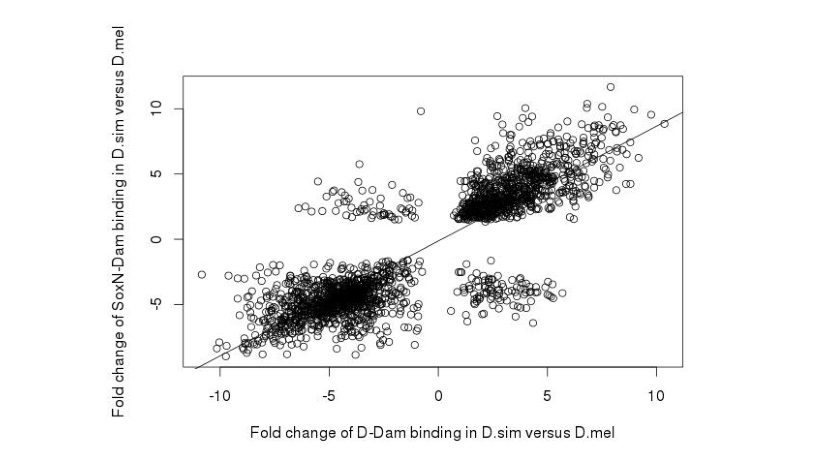
\includegraphics{fig5-26}
\caption{Scatter plot of fold changes between binding in \emph{D. melanogaster} and \emph{D. simulans} for Dichaete-Dam versus for SoxN-Dam in intervals bound by both TFs that are differentially bound between species. Positive fold changes indicate preferential binding in \emph{D. simulans}, while negative fold changes indicate preferential binding in \emph{D. melanogaster}. Most differentially bound intervals are more strongly bound in the same species by both Dichaete-Dam and SoxN-Dam, while a smaller number are more strongly bound in different species by each TF. Similar numbers of intervals are preferentially bound in each species overall.}
\label{Figure 5.26}
\end{figure}

\section{Evolutionary analysis of Sox binding motifs}
The availability of sequence data and \emph{in vivo} binding data for each species facilitates an analysis of the contributions of sequence conservation within binding intervals and at TF-specific binding motifs to qualitative and quantitative binding conservation. In order to examine the patterns of motif conservation, I first identified all matches to the best \emph{de novo} Sox motif discovered in each set of binding intervals using the tool FIMO \citep{grant_fimo:_2011}, with a p-value cutoff of 1e-4. I did the same with intervals that had been randomly shuffled to different locations in each genome using the BEDTools shuffle utility, as a control for each dataset \citep{quinlan_bedtools:_2010}. These shuffled intervals have the same lengths as the original binding intervals. The mean numbers of Sox motifs per binding interval range from 1.19 in the \emph{D. pseudoobscura} Dichaete-Dam intervals to 2.75 in the \emph{D. yakuba} Dichaete-Dam intervals. In all cases, there are significantly more Sox motifs in binding intervals than in randomly shuffled control intervals (p \textless 4.03e-15, Wilcoxon rank sum test with continuity correction). For the following analyses, I focused on Dichaete-Dam, comparing binding intervals showing four-way conservation between all species studied with intervals that are unique to \emph{D. melanogaster}. I found 1896 \emph{D. melanogaster} binding intervals that are conserved in all four species. These highly conserved intervals have significantly more Sox motifs on average (mean = 4.53) than do unique \emph{D. melanogaster} binding intervals (mean = 1.29, p = 3.03e-193, Wilcoxon rank sum test with continuity correction) (Figure 5.27A).\\

Using PRANK, a phylogeny-aware aligner, I created multiple alignments of the orthologous sequences in each species for both the four-way conserved binding intervals and the unique \emph{D. melanogaster} binding intervals \citep{loytynoja_algorithm_2005,loytynoja_phylogeny-aware_2008}. I only considered intervals for which a high-confidence orthologous sequence could be identified in all four species, which reduced the sets of intervals to 1064 showing four-way binding conservation and 1560 showing unique binding in \emph{D. melanogaster}. These sequences should contain the enhancers or regulatory DNA to which Dichaete binds; however, they also contain flanking regions which may not be of functional relevance. Not surprisingly, the intervals showing four-way binding conservation do not display a higher rate of nucleotide conservation on average than the unique \emph{D. melanogaster} intervals \citep{he_high_2011}. In fact, the uniquely-bound intervals are slightly, but significantly, more conserved across their entire lengths (Wilcoxon p = 2.337e-20) (Figure 5.27B).\\

I scanned each set of multiple alignments for matches to the \emph{de novo} Sox motifs, resulting in a count of the number of motifs in each binding interval that are positionally conserved in all four species as well as the nucleotide conservation within each motif. Within the set of intervals that show four-way binding conservation, 20.1\% of all motifs identified in \emph{D. melanogaster} are positionally conserved in all four species, with 19.5\% of motifs in each interval being conserved on average. In the set of intervals that are only bound in \emph{D. melanogaster}, 16.2\% of all motifs identified in \emph{D. melanogaster} are positionally conserved in all four species, with 16.1\% of motifs in each interval being conserved on average (Figure 5.27C). A similar pattern holds when examining only those motifs that are both positionally conserved and that show 100\% nucleotide conservation. In this case, for the intervals showing four-way binding conservation, 15.6\% of all motifs identified in \emph{D. melanogaster} show complete conservation (positional and sequence) in all four species, with 14.9\% of motifs in each interval being conserved on average. For the intervals that are uniquely bound in \emph{D. melanogaster}, 12.6\% of all motifs identified in \emph{D. melanogaster} show complete conservation, with 12.4\% of motifs in each interval being conserved on average (Figure 5.27D). The differences in conservation rates between motifs in intervals showing four-way binding conservation and those uniquely bound in \emph{D. melanogaster} are significant for both positional conservation (Wilcoxon p = 2.55e-24) and combined positional and nucleotide conservation (Wilcoxon p = 6.04e-28).\\

The Sox motifs identified in \emph{D. melanogaster} binding intervals show high levels of nucleotide conservation in all four species overall, regardless of whether the orthologous sequences were identified as motif matches in other species or not. In the set of intervals showing four-way binding conservation, 14147 Sox motifs were identified in \emph{D. melanogaster} that could be aligned without gaps to orthologous sequences in each other species. These motifs show an average of 74.5\% nucleotide conservation across all four sequences in the multiple alignments. In the set of intervals showing unique binding in \emph{D. melanogaster}, 5204 Sox motifs were identified in \emph{D. melanogaster} that could be aligned without gaps to orthologous sequences in each other species. These motifs show a lower average nucleotide conservation, 69.9\%. The difference in motif nucleotide conservation rates between intervals showing four-way binding conservation and those uniquely bound in \emph{D. melanogaster} is significant according to a Wilcoxon rank-sum test (p = 9.56e-36). As a further control, I randomly shuffled the columns in each PWM to produce a set of control motifs with the same GC content and length as the Sox motifs and searched for matches to each of them in the multiply aligned binding intervals. The average rates of nucleotide conservation are similar for shuffled control motifs in both sets of intervals, although they are slightly higher in intervals that display four-way binding conservation (70.7\% versus 67.2\% for unique \emph{D. melanogaster} intervals, Wilcoxon p = 2.07e-19). The differences between average nucleotide conservation in Sox motifs and control motifs in both the four-way conserved binding intervals and the unique \emph{D. melanogaster} binding intervals are also significant (Wilcoxon p = 1.62e-43
 and p = 1.67e-9). Out of each set of motifs examined, the Sox motifs in intervals with four-way binding conservation clearly show the highest nucleotide conservation (Figure 5.27E).\\

\begin{figure}[H]
\centering
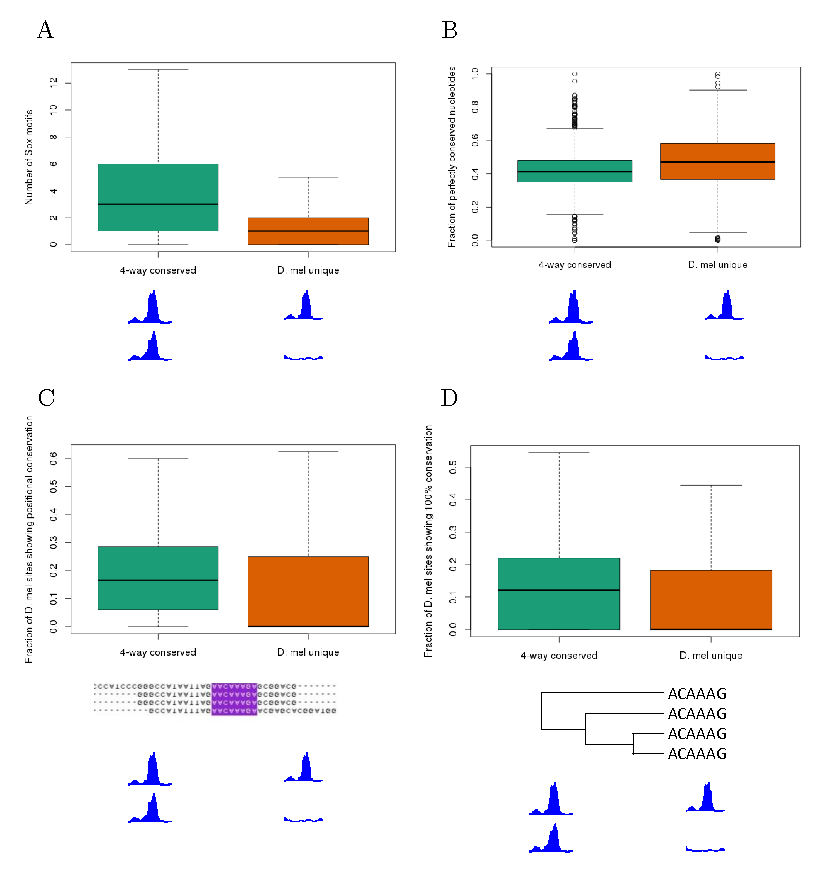
\includegraphics{fig5-27a}
\label{Figure 5.27}
\end{figure}

\begin{figure}[H]
\centering
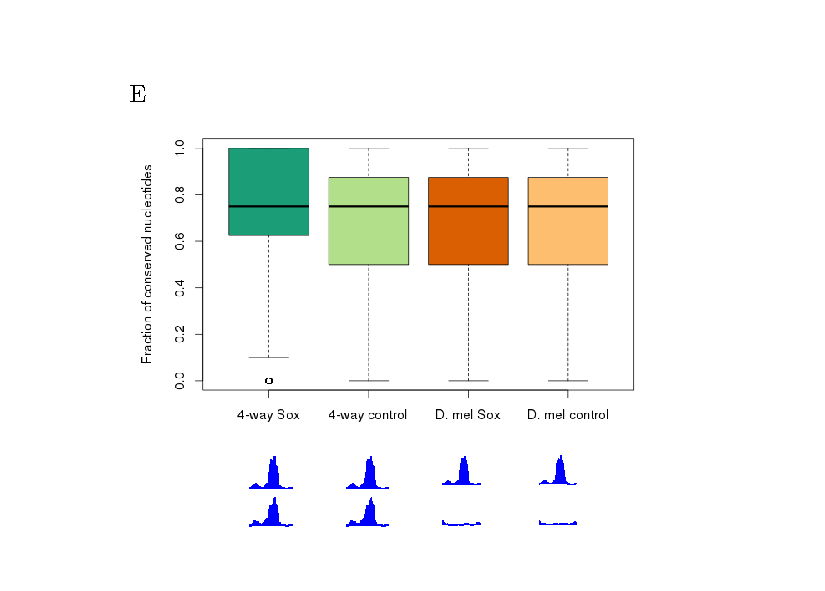
\includegraphics{fig5-27e}
\caption{Number and conservation of Sox motifs are associated with binding conservation. A.) On average, Dichaete-Dam binding intervals that are conserved between all four species have more Sox motifs than intervals that are unique to \emph{D. melanogaster} (p = 3.03e-193). B.) Dichaete-Dam binding intervals that are conserved between all four species do not show a greater fraction of total nucleotide conservation on average than intervals that are unique to \emph{D. melanogaster}. C.) On average, Dichaete-Dam binding intervals that show four-way binding conservation have more positionally conserved Sox motifs than intervals that are only bound in \emph{D. melanogaster} (p = 2.55e-24 ). D.) On average, Dichaete-Dam binding intervals that show four-way binding conservation have more Sox motifs with 100\% nucleotide conservation in addition to positional conservation than intervals that are only bound in \emph{D. melanogaster} (p = 6.04e-28). E.) On average, Sox motifs in Dichaete-Dam intervals that are bound in all four species (“4-way Sox”) have a greater percentage of perfectly conserved nucleotides than either Sox motifs in intervals that are only bound in \emph{D. melanogaster} (“D. mel Sox”, p = 9.56e-36), randomly shuffled control motifs in intervals that are bound in all four species (“4-way control”, p = 1.62e-43) or randomly shuffled control motifs in intervals that are only bound in \emph{D. melanogaster} (“D. mel control”, p = 1.67e-9).}
\label{Figure 5.27}
\end{figure}

For binding intervals that are conserved but show quantitative changes in affinity in pairwise comparisons, I wanted to test whether motif quality was correlated with binding affinity. This has been shown to be the case for Bcd in a comparison between \emph{D. melanogaster, D. yakuba, D. pseudoobscura} and \emph{D. virilis}, as well as for Twi in a comparison between \emph{D. melanogaster, D. simulans, D. yakuba, D. erecta, D. ananassae} and \emph{D. pseudoobscura} \citep{he_high_2011,paris_extensive_2013}. I used two strategies to examine this question. First, I searched for Sox motifs in all Dichaete-Dam and SoxN-Dam intervals that were conserved but differentially bound between pairs of species using FIMO \citep{grant_fimo:_2011}. FIMO reports motif scores in the GFF output files which are calculated as -10*(log10(p-value)), thus reflecting the statistical confidence that a given sequence matches the consensus motif. In cases where more than one motif is predicted within an interval, it is difficult to determine a priori which motif(s) are primarily responsible for TF binding, since DamID binding intervals are not necessarily centered around the binding site. I therefore found both the average motif score and the total (cumulative) motif score within each interval in each species examined. Performing a linear regression of the log2 fold change in binding affinity between each pair of species at each interval versus the difference in either average or cumulative motif score at each interval reveals no significant correlations between motif quality and quantitative changes in binding, the one exception being for average motif scores in differentially bound SoxN-Dam intervals between \emph{D. melanogaster} and \emph{D. simulans}, where a weak but significant correlation is present (R\textsuperscript{2} = 0.0027, p = 0.0057) (Figure 5.28).\\

\begin{figure}[H]
\centering
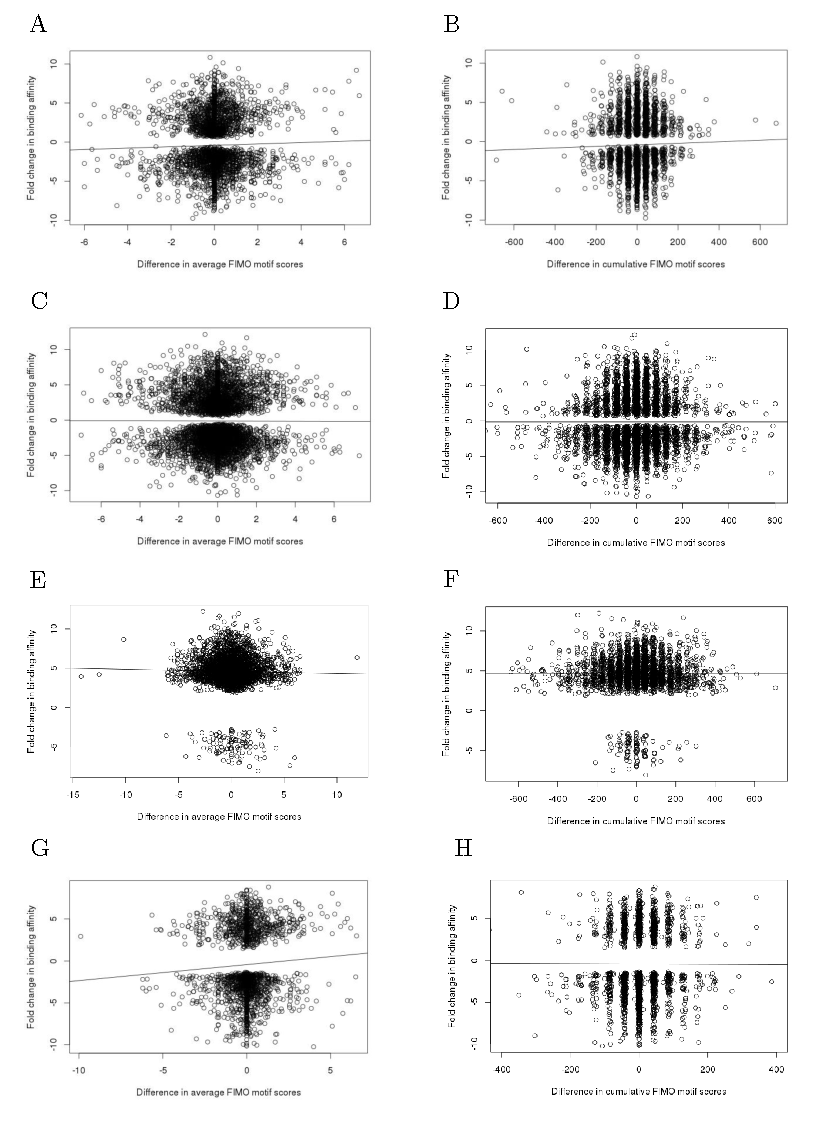
\includegraphics{fig5-28}
\label{Figure 5.28}
\end{figure}

\begin{figure}[H]
\centering
\caption{Changes in Sox motif quality within binding intervals between species do not correlate with changes in group B Sox binding affinity. Differences in cumulative or average motif scores between species are plotted on the x-axis and differences in binding affinity are plotted on the y-axis. Positive binding affinity and motif score differences represent increased binding or motif quality in \emph{D. melanogaster}, while negative fold changes and negative motif score differences represent increased binding or motif quality in each other species. A.) Log2 fold change of Dichaete-Dam binding in \emph{D. melanogaster} versus \emph{D. simulans} plotted against the difference between average \emph{D. melanogaster} motif scores and average \emph{D. simulans} motif scores in each interval. R\textsuperscript{2} = 0.00046, p = 0.099. B.) Log2 fold change of binding in \emph{D. melanogaster} versus \emph{D. simulans} plotted against the difference between cumulative \emph{D. melanogaster} motif scores and cumulative \emph{D. simulans} scores in each interval. R\textsuperscript{2} = 0.00014, p = 0.21. C.) Log2 fold change of Dichaete-Dam binding in \emph{D. melanogaster} versus \emph{D. yakuba} plotted against the difference between average \emph{D. melanogaster} motif scores and average \emph{D. yakuba} motif scores in each interval. R\textsuperscript{2} = -0.00016, p = 0.86. D.) Log2 fold change of Dichaete-Dam binding in \emph{D. melanogaster} versus \emph{D. yakuba} plotted against the difference between cumulative \emph{D. melanogaster} motif scores and cumulative \emph{D. yakuba} motif scores in each interval. R\textsuperscript{2} = -7.95e-05, p = 0.47. E.) Log2 fold change of Dichaete-Dam binding in \emph{D. melanogaster} versus \emph{D. pseudoobscura}  plotted against the difference between average \emph{D. melanogaster} motif scores and average \emph{D. pseudoobscura} motif scores in each interval. R\textsuperscript{2} =  0.00014, p = 0.22.  F.) Log2 fold change of Dichaete-Dam binding in \emph{D. melanogaster} versus \emph{D. pseudoobscura}  plotted against the difference between cumulative \emph{D. melanogaster} motif scores and cumulative \emph{D. pseudoobscura} motif scores in each interval. R\textsuperscript{2} =  -0.00028, p = 0.85. G.) Log2 fold change of SoxN-Dam binding in \emph{D. melanogaster} versus \emph{D. simulans} plotted against the difference between average \emph{D. melanogaster} motif scores and average \emph{D. simulans} motif scores in each interval. R\textsuperscript{2} = 0.0027, p = 0.0057). H.) Log2 fold change of SoxN-Dam binding in \emph{D. melanogaster} versus \emph{D. simulans} plotted against the difference between cumulative \emph{D. melanogaster} motif scores and cumulative \emph{D. simulans} motif scores in each interval. R\textsuperscript{2} =  -7.41e-05, p = 0.37).}
\label{Figure 5.28}
\end{figure}
 
As a secondary strategy, I found the scores assigned by RSAT to all positionally conserved motifs identified in four-way conserved Dichaete-Dam binding intervals that had been multiply aligned. The majority of these motifs have identical sequences and thus the same score in all species; however, there are some cases where a mutation in one species leads to a better or worse match to the consensus motif. For each pairwise comparison between species, I divided the intervals by whether they showed differential binding in one species or the other and counted the number of motifs in each group of intervals that had a higher score in each species. I compared the number of motifs in intervals that have a higher score in the species in which the interval is preferentially bound with the number of motifs that have a lower score in the species in which the interval is preferentially bound. Comparing \emph{D. melanogaster} and \emph{D. simulans}, there are more total Sox motifs that score higher in \emph{D. melanogaster} than Sox motifs that score lower in \emph{D. melanogaster} in intervals that are preferentially bound in that species (26 versus 14), and the same holds true for \emph{D. simulans} (5 versus 2). However, this pattern does not hold for the comparison of \emph{D. melanogaster} and \emph{D. yakuba}; in intervals preferentially bound in \emph{D. melanogaster}, there are 35 motifs that score more highly in that species and 40 that score more highly in \emph{D. yakuba}, while in intervals preferentially bound in \emph{D. yakuba}, there are 26 motifs that score more highly in that species and 25 that score more highly in \emph{D. melanogaster}. Comparing \emph{D. melanogaster} and \emph{D. pseudoobscura}, in intervals that are more highly bound in \emph{D. melanogaster}, there are 189 motifs that score more highly in that species versus 173 that score more highly in \emph{D. pseudoobscura}, while only one motif scoring more highly in each species was found in intervals that are preferentially bound in \emph{D. pseudoobscura}. Counting the number of motifs within each interval, rather than the total number of motifs found for each group of intervals, there are no significant differences between the numbers of higher-scoring motifs and lower-scoring motifs in intervals that are preferentially bound in any pairwise species comparison (\emph{D. melanogaster} vs. \emph{D. simulans}, p = 0.48; \emph{D. melanogaster} vs. \emph{D. yakuba}, p = 0.45; \emph{D. yakuba} vs. \emph{D. melanogaster}, p = 0.18; \emph{D. melanogaster} vs. \emph{D. pseudoobscura}, p = 0.64).\\

Given the correlation between motif conservation and qualitative binding conservation, it is somewhat surprising to find no detectable correlation between motif quality and quantitative changes in binding affinity. However, in the case of four-way positionally conserved motifs, such an effect might be obscured by the high overall degree of quality and nucleotide conservation in the motifs examined. The FIMO motif analysis, in which all motifs in four-way conserved binding intervals were scored, should uncover a broader range of variability in motif quality; however, in this case, the fact that the scores of all motifs in each interval were taken into account, either through averaging or examining the cumulative motif scores, could obscure a signal from one or a few motifs that have a more direct effect on TF binding. The Twi study, which used ChIP-seq data, focused on the quality of motifs within a 151-bp window around the binding peak summit \citep{he_high_2011}, allowing for a more focused assessment of the effect of motif quality on binding. However, in DamID binding intervals, the highest scoring nucleotide does not necessarily correspond to the center of TF binding, due to the non-random distribution of GATC sites in the genome. This makes it difficult to narrow down binding regions in order to identify motifs that might be the most relevant for binding. Additionally, the technical differences between DamID and ChIP may make ChIP a more sensitive measure of quantitative binding affinity than DamID; this has not been tested experimentally. Nonetheless, the analyses of qualitative binding conservation show that both the number of Sox motifs in an interval and the positional and nucleotide conservation levels of those motifs are correlated with conserved binding.

\section{Discussion of results}
In this chapter, I set out to analyze the binding patterns of Dichaete and SoxN in the context of \emph{Drosophila} evolution, using the DamID datasets that I generated. First, I performed quantitative binding comparisons between each pair of species for each TF. Normalizing the read counts from all samples in each pair of species together allowed me to reduce the effects of comparing separately thresholded samples, which can lead to an underestimate of similarity. Since the identification of differentially bound intervals by DiffBind requires a list of bound intervals in each sample as input, there is still some potential for thresholding effects. Nonetheless, pooling the bound intervals from all samples before the differential enrichment analysis should minimize this problem. The percentages of \emph{D. melanogaster} binding intervals detected as qualitatively or quantitatively divergent between emph{D. melanogaster} and each other species range from 21.4\% for SoxN-Dam in \emph{D. simulans} to 44.2\% for Dichaete-Dam in \emph{D. yakuba}. On the level of read counts, the binding affinity score correlations in bound regions for the same TF between \emph{D. melanogaster} and \emph{D. simulans} range from 0.62 - 0.72 for Dichaete-Dam and from 0.75 - 0.90 for SoxN-Dam. For Dichaete-Dam between \emph{D. melanogaster} and \emph{D. yakuba}, they range from 0.68 - 0.70, and for Dichaete-Dam between \emph{D. melanogaster} and \emph{D. pseudoobscura}, they are more variable, ranging from 0.46 - 0.72. These numbers are in line with correlations of AP factor binding between \emph{D. melanogaster} and \emph{D. yakuba}, which range from 0.57 for Cad to 0.75 for Kr \citep{radley_binding_2010}. The quantitative changes in Dichaete binding between each pair of species examined follow the known \emph{Drosophila} phylogeny \citep{russo_molecular_1995}, with greater differences detected between more distant species, which follows an expectation of neutral evolution according to a molecular clock mechanism \citep{he_high_2011}.\\

The reduced quality of the \emph{D. pseudoobscura} Dichaete-Dam samples compared to those from the other species and the consequent lower number of binding intervals called in \emph{D. pseudoobscura} posed a challenge for further analysis. In order to make a quantitative comparison between Dichaete-Dam binding in \emph{D. pseudoobscura} and \emph{D. melanogaster}, I decided to normalize the samples by total library size rather than by read counts in bound regions, since the numbers of bound regions were so different between the two species. This approach is a conservative one and may have underestimated the number of intervals that are preferentially bound in \emph{D. pseudoobscura}; however, it prevented the over-inflation of binding signal in the \emph{D. pseudoobscura} samples. For the subsequent analyses of binding conservation in relation to functional annotations, I decided to focus on a three-way comparison of Dichaete-Dam binding in \emph{D. melanogaster, D. simulans} and \emph{D. yakuba}, as these datasets are of comparable quality and offer the most unbiased view of evolutionary differences across the \emph{melanogaster} clade. Normalizing samples from these three species together revealed a similar pattern of binding divergence as that seen in pairwise comparisons and confirmed the fact that changes in Dichaete-Dam binding correspond with the \emph{Drosophila} phylogeny.\\

Besides quantitative and qualitative conservation of binding at orthologous loci between species, a comparative study of TF binding can be used to address the question of compensatory evolution or binding site turnover, when binding events evolve at different positions between species but regulate the same gene. Without gene expression data or functional enhancer assays, it is impossible to prove which binding events have a direct effect on gene regulation; nonetheless, by annotating binding events that are not positionally conserved to genes, I identified potential instances of Dichaete and SoxN binding site turnover between \emph{D. melanogaster} and \emph{D. simulans} as well as between \emph{D. melanogaster} and \emph{D. yakuba}. These binding events represent a large proportion of non-positionally conserved binding intervals between species. In \emph{D. simulans}, out of 4472 Dichaete-Dam binding intervals that are not positionally conserved in \emph{D. melanogaster}, 3226 or 72.1\% are potential instances of binding site turnover, while conversely, 58.2\% of \emph{D. melanogaster} Dichaete-Dam intervals that are not positionally conserved in \emph{D. simulans} could represent binding site turnover. For SoxN-Dam, the non-positionally conserved intervals that are identified as showing compensatory conservation represent 90.4\% of \emph{D. simulans} binding intervals and 61.4\% of \emph{D. melanogaster} binding intervals. Comparing Dichaete-Dam binding in \emph{D. melanogaster} and \emph{D. yakuba}, they represent 79.5\% of \emph{D. yakuba} non-positionally conserved intervals and 78.5\% of \emph{D. melanogaster} non-positionally conserved intervals. This supports the view that Dichaete and SoxN have very similar gene targets in each species studied, since in the majority of instances where binding has been lost in one species, a separate binding site has been gained at the same gene locus.\\

The availability of STARR-seq enhancer activity maps in several species of \emph{Drosophila} allows for an interesting comparison of TF binding conservation with overall enhancer conservation \citep{arnold_genome-wide_2013}. Applying the same criteria that I used for Dichaete and SoxN binding sites, I identified STARR-seq enhancers in \emph{D. melanogaster} and \emph{D. yakuba} that show compensatory conservation. Although a large number of enhancers show evidence of turnover, relatively few of them are bound by Dichaete-Dam in either \emph{D. melanogaster} or \emph{D. yakuba}. Even fewer contain a Dichaete-Dam binding site in either species that also shows compensatory conservation. Of all the Dichaete-Dam binding intervals that are potential instances of binding site turnover, only 1.1\% and 2.1\% of \emph{D. melanogaster} intervals are located in STARR-seq enhancers that show turnover in S2 cells or OSCs, respectively, and only 1.8\% and 3.1\% of \emph{D. yakuba} intervals are located in STARR-seq enhancers that show turnover in S2 cells or OSCs. Although binding site turnover at gene loci appears to be a common mode of evolution for Dichaete and SoxN in \emph{Drosophila}, new binding events are not generally gained in newly-evolved enhancers, but rather in enhancer regions whose regulatory activity is conserved between species. This finding, although initially surprising, is in line with the hypothesis that turnover of TF binding events should operate to maintain the level of transcriptional output of their target enhancers under balancing selection.\\

The other sources of annotated enhancers that I used in this study, REDFly and FlyLight, do not have comparative data available \citep{gallo_redfly_2010,manning_resource_2012}. However, given the high overlap that I found between \emph{D. melanogaster} binding intervals and these enhancers, I was curious about the relationship between binding in validated enhancers and binding conservation. I found a strong correlation between the two; for Dichaete-Dam, \emph{D. melanogaster} binding events that overlap with an enhancer from either database are more likely to be conserved in both \emph{D. simulans} and \emph{D. yakuba}, while for SoxN-Dam, they are more likely to be conserved in \emph{D. simulans}. For both TFs, binding intervals that overlap with a REDFly or FlyLight enhancer are less likely to be unique to \emph{D. melanogaster} (Figure 5.19). This result confirms that binding to known functional regions is subject to selective pressure and is therefore more likely to be maintained during evolution. Interestingly, an even stronger effect was observed for binding intervals that overlap with a Dichaete or SoxN core interval (Figure 5.20) \citep{aleksic_role_2013,ferrero_soxneuro_2014}. While the core intervals were defined by overlapping multiple \emph{D. melanogaster} genome-wide binding datasets, including ChIP-seq and DamID, their evolutionary conservation has not previously been assessed. The fact that DamID binding events that overlap with core intervals are much more likely to be conserved across all species studied than those that do not provides strong evidence for the importance of these binding intervals in group B Sox function. A smaller, but still significant, effect was found for binding intervals that are annotated to known Dichaete and SoxN target genes (Figure 5.21) \citep{aleksic_role_2013,ferrero_soxneuro_2014}. It should be noted that very conservative criteria were used to define direct target genes; for example, bound genes that show modest expression changes in mutant embryos were excluded. Such genes would include bona fide Sox targets whose expression is rescued by functional compensation. Hence it is likely that the true fraction of conserved target genes is higher than reported here.\\

The availability of a sequenced genome for all four species studied allowed me to examine the connection between binding intervals sequence motif content and \emph{in vivo} binding conservation \cite{clark_evolution_2007}. Previous comparative studies using ChIP-seq have found that overall nucleotide conservation is not significantly elevated in binding intervals that are conserved between species \citep{bradley_binding_2010,he_high_2011}. Since DamID binding intervals tend to be wider than ChIP-seq intervals and are not centered on the binding site, my expectation was that this would hold true in my DamID data. Indeed, I found no correlation between binding conservation and increased nucleotide conservation across the entire intervals. However, I did find significant correlations between binding conservation and several measures of Sox motif content. First, conserved intervals have more matches to Sox motifs on average than non-conserved intervals or control intervals whose genomic coordinates were randomly shuffled. This indicates that an increased density of recognizable motifs may contribute to group B Sox binding function and be important for its conservation. On the level of individual motifs, intervals with conserved binding contain more matches to Sox motifs that show positional conservation within the interval as well as showing 100\% nucleotide conservation between species. Matches to Sox motifs within intervals that show conserved binding also have a higher percentage of conserved nucleotides than those in intervals that do not show conserved binding or than matches to control motifs whose columns were randomly shuffled. It is difficult to say whether higher quality Sox motifs lead to more functional binding or whether functional binding leads to selective pressure on Sox motifs; however, it seems likely that a feedback mechanism might act to maintain the observed correlation between highly conserved motif matches and \emph{in vivo} binding conservation.\\

In the previous chapter, I began to address the question of common and unique binding by Dichaete and SoxN in \emph{D. melanogaster} and \emph{D. simulans}, noting that the binding patterns of the two Dam fusions appear more similar in \emph{D. melanogaster}. Here I have explored the evolutionary relationship between these two TFs in more detail. The most striking observation from my analysis is the strong association between common binding by Dichaete and SoxN and binding conservation. Intervals that show binding by both TFs in one species are much more likely to be bound in the other species, and specifically to also be bound by both TFs in that species. Conversely, of the intervals that are uniquely bound by either Dichaete or SoxN in one species, relatively few are also uniquely bound by the same TF in the other species, suggesting that unique binding by one TF is less constrained by selection than common binding. A large number of intervals that are bound by one TF in \emph{D. simulans} are bound by both in \emph{D. melanogaster}, supporting the original observation that Dichaete-Dam and SoxN-Dam binding patterns are more similar in \emph{D. melanogaster}. It is unclear why this is the case; however, given the fact that a higher percentage of \emph{D. simulans} commonly-bound intervals are conserved in \emph{D. melanogaster} than vice versa, the intervals that are commonly bound in both species could represent a core set of binding intervals are likely to be of key functional importance.\\

Although I found a high level of conservation of common binding by Dichaete and SoxN, there are also examples of unique binding that are conserved in both species, which can be used to examine the conserved functions that are specific to each TF. Using both these data and a DiffBind analysis that searched for differentially bound intervals between the two TFs using data from both species normalized together, I identified target genes that are uniquely bound by either Dichaete or SoxN in both species. Functional enrichment analyses using Flymine indicated that the major differences between these sets of target genes are in the tissues in which they are expressed, rather than biological processes in which they play a role. Specifically, conserved, unique Dichaete targets are upregulated in a broader range of tissues than conserved, unique SoxN targets, including the head, brain, crop and hindgut. The presence of unique Dichaete targets in the brain and hindgut is particularly interesting, as Dichaete is known to play a role in the development of these tissues \citep{sanchez-soriano_regulatory_2000}. Additionally, a strong motif for Byn, a TF that is critical for hindgut development \citep{kispert_homologs_1994,murakami_developmental_1999}, was found in conserved, uniquely-bound Dichaete intervals, suggesting that Dichaete and Byn might work together to regulate target gene expression in the hindgut. This motif was not identified in single-species analyses or in an analysis of the entire set of Dichaete-bound intervals, highlighting the power of a comparative analysis to detect specific features of regulatory function. In the case of SoxN, conserved, uniquely-bound targets are largely expressed in the CNS. The presence of a Usp motif in these intervals and the enrichment of target genes in the Robo-Slit signalling pathway highlight a conserved role for SoxN in axon morphogenesis and pathfinding \citep{ferrero_soxneuro_2014,girard_chromatin_2006,lee_cell-autonomous_????,parrish_genome-wide_2006}.\\

Taken together, these results suggest a model whereby Dichaete and SoxN binding, while subject to turnover during evolution, is highly conserved at loci where both TFs can bind and at potentially functional sites, including annotated enhancers and core Dichaete and SoxN intervals. Given the similarity of the motifs recognized by these two TFs and the number of target genes that they share, it may be easier for natural selection to maintain sites where both Dichaete and SoxN can bind, rather than maintaining independent binding sites for each. From another perspective, sequences that can be bound and contribute to functional regulation by both Dichaete and SoxN may experience a double dose of selective constraint. If this were true, then why would sites that are uniquely bound by one TF be conserved at all? The comparative data suggest that conserved, uniquely bound targets are largely expressed in different tissues, corresponding to the differences in expression patterns shown by Dichaete and SoxN themselves. At loci where Dichaete and SoxN have evolved new, independent regulatory functions, unique binding could be driven by external factors such as differences in chromatin accessibility between embryonic tissues or the availability of cofactors that might interact specifically only one Sox protein, which would prevent the other protein from binding in tissues in which they are commonly expressed. In the following chapters, I will explore the question of chromatin accessibility in \emph{D. pseudoobscura} and its relationship to group B Sox binding and then conclude by attempting to synthesize the information gained from my comparative studies of chromatin accessibility and transcription factor binding.  

